%
\documentclass[11pt]{article}
\newcommand{\teilnr}{II}
\usepackage{xr}
\externaldocument{../teil1/main_teil1}
\externaldocument{../teil3/main_teil3}
%
%
\usepackage[margin=1.2in]{geometry}
\usepackage{graphicx}
%
\makeatletter\newcommand*{\captionfigur}{\def\@captype{figure}\caption}\makeatother
\usepackage{tikz}\usetikzlibrary{fit,calc,arrows.meta,backgrounds}   %
%
\renewcommand{\topfraction}{0.85}\renewcommand{\textfraction}{0.1}\renewcommand{\floatpagefraction}{0.75}
\graphicspath{{../abbildungen/}}   %
\usepackage[T1]{fontenc}
\usepackage{lmodern}
\usepackage{amsmath,amssymb,amsthm}
\usepackage{etoolbox}
\usepackage{refcount}
\usepackage{array}       %
\usepackage{longtable}   %
\usepackage[hidelinks]{hyperref}

\providecommand{\teilnr}{?}
\newif\ifimband

%
\newtheorem{theorem}{Theorem}[section]
\newtheorem{proposition}[theorem]{Proposition}
\newtheorem{lemma}[theorem]{Lemma}
\newtheorem{corollary}[theorem]{Corollary}
\theoremstyle{definition}
\newtheorem{definition}[theorem]{Definition}
\theoremstyle{remark}
\newtheorem{remark}[theorem]{Remark}
\newtheorem{question}[theorem]{Question}
\renewcommand{\thetheorem}{\teilnr.\arabic{section}.\arabic{theorem}}
\numberwithin{equation}{section}
%
%
\def\theHtheorem{\teilnr.\arabic{section}.\arabic{theorem}}
\def\theHsection{\teilnr.\arabic{section}}
\def\theHequation{\teilnr.\arabic{section}.\arabic{equation}}

%
%
%
%
\newcommand{\tlabel}[1]{\label{\teilnr:#1}}
%
%
%
\newwrite\belegaus
\immediate\openout\belegaus=\jobname.bel
\newcommand{\belegart}[1]{\immediate\write\belegaus{\thetheorem|#1|\thesection}{\normalfont\small[#1]}\ }
\newcommand{\tref}[1]{\ref{\teilnr:#1}}
\makeatletter
\newcommand{\partref}[2]{%
  \edef\serie@teil{\teilnr}\def\serie@ziel{#1}%
  \ifx\serie@teil\serie@ziel\ref{#1:#2}%
  \else\ifimband\ref{#1:#2}%
  \else\getrefnumber{#1:#2}~in~[Part~#1]\fi\fi}
\makeatother

%
%
%
%
\makeatletter
%
\@namedef{Z@nenner}{811}
%
\@namedef{Z@offen}{6}
%
\@namedef{Z@erledigt}{805}
%
\@namedef{Z@zertifiziert}{767}
%
\@namedef{Z@vollzerlegt}{38}
%
\@namedef{Z@csechsquadrat}{1.3685}
%
\@namedef{Z@csechswalker}{0.3137}
%
\@namedef{Z@csechs}{1.6822}
%
\@namedef{Z@streifenfam}{206}
%
\@namedef{Z@streifentot}{52}
%
\@namedef{Z@streifentuerme}{154}
%
\@namedef{Z@streifenstellen}{8.4\cdot 10^{7}}
%
\@namedef{Z@streifenminm}{223}
%
\@namedef{Z@streifensieben}{17.5}
%
\@namedef{Z@streifeneins}{2}
%
\@namedef{Z@margestich}{530}
%
\@namedef{Z@margemax}{10^{8}}
%
\@namedef{Z@margerand}{2\cdot 10^{5}}
%
\@namedef{Z@margemin}{21.5}
%
\@namedef{Z@streifenschranke}{2000}
%
\@namedef{Z@streifensteckt}{14}
%
\@namedef{Z@glattkerne}{889\,437}
%
\@namedef{Z@glattkand}{0}
%
\@namedef{Z@glattunten}{10^{8}}
%
\@namedef{Z@glattoben}{10^{15}}
%
\@namedef{Z@glatthoehe}{2000}
%
\@namedef{Z@glattprim}{100}
%
\@namedef{Z@glattmin}{4}
%
\@namedef{Z@glattperiode}{9573}
%
\@namedef{Z@glattgross}{356\,888}
%
\@namedef{Z@glattrest}{532\,549}
%
\@namedef{Z@bboxkern}{10^{6}}
%
\@namedef{Z@bboxb}{10^{4}}
%
\@namedef{Z@bboxfam}{101\,329}
%
\@namedef{Z@bboxparitaet}{32\,118}
%
\@namedef{Z@bboxpaare}{421\,010\,513}
%
\@namedef{Z@bboxohnealpha}{343\,504\,538}
%
\@namedef{Z@bboxzweiadisch}{16\,603\,302}
%
\@namedef{Z@bboxkgerade}{11\,242\,224}
%
\@namedef{Z@bboxlemmal}{49\,659\,524}
%
\@namedef{Z@bboxrest}{925}
%
\@namedef{Z@ballotfaelle}{56}
%
\@namedef{Z@ballotgedruckt}{0}
%
\@namedef{Z@ballotfib}{50}
%
\@namedef{Z@turmk1}{1.1\cdot 10^{13}}
%
\@namedef{Z@turmk2}{5.5\cdot 10^{13}}
%
\@namedef{Z@turmk3}{4.5\cdot 10^{30}}
%
\@namedef{Z@turmstellen}{2.5\cdot 10^{15}}
%
\@namedef{Z@kongruenzbis}{10^{5}}
%
\@namedef{Z@kongruenzdichte}{2.67\cdot 10^{-4}}
%
\@namedef{Z@yokoimax}{20000}
%
\@namedef{Z@yokoipaare}{123}
%
\@namedef{Z@designkerne}{251}
%
\@namedef{Z@designtmax}{399}
%
\@namedef{Z@designfenster}{17}
%
\@namedef{Z@designmaxm}{1023}
%
\@namedef{Z@designstellen}{2000}
%
\@namedef{Z@quadratzeuge1}{701}
%
\@namedef{Z@quadratzeuge2}{3}
%
\@namedef{Z@quadratzeuge3}{5}
%
\@namedef{Z@mittenquadrat}{0.3648}
%
\@namedef{Z@mittendoppel}{0.2580}
%
\@namedef{Z@mittensatza}{0.6228}
%
\@namedef{Z@mittenN}{10^{14}}
%
\@namedef{Z@mittengemessen}{0.6252}
%
\@namedef{Z@kerne}{10\,132\,126}
%
\@namedef{Z@kernschranke}{10^{8}}
%
\@namedef{Z@hoehe}{2000}
%
\@namedef{Z@zeugenschranke}{2\cdot 10^{5}}
%
\@namedef{Z@filterfamilien}{83}
%
\@namedef{Z@punktfamilien}{79}
%
\@namedef{Z@punkte}{445}
%
\@namedef{Z@paritaetspunkte}{74}
%
\@namedef{Z@zeugenpunkte}{371}
%
\@namedef{Z@restpunkte}{0}
%
\@namedef{Z@beispielm}{7}
%
\@namedef{Z@beispielk}{7}
%
\@namedef{Z@beispielzeuge}{29}
%
\@namedef{Z@beispielwert}{130\,576\,328}
%
\@namedef{Z@beispielfaktoren}{2^{3}\cdot 29\cdot 197\cdot 2857}
%
\@namedef{Z@ohnetripel}{3.88\cdot 10^{20}}
%
\@namedef{Z@ohnetripelsicher}{1.83\cdot 10^{18}}
%
\@namedef{Z@famtab}{(2, 1) & 1 & 0.90 & 1.53 & 14 \\
(3, 1) & 3 & 2.83 & 3.43 & 6 \\
(23, 2) & 1 & 4.09 & 9.37 & 2 \\
(6, 1) & 3 & 5.37 & 5.97 & 3 \\
(1, 5) & 5 & 5.67 & 12.54 & 2 \\
(46, 1) & 1 & 8.77 & 9.37 & 2 \\
(7, 2) & 7 & 9.73 & 20.67 & 1 \\
(5, 1) & 5 & 11.94 & 12.54 & 1 \\
(430, 1) & 1 & 12.91 & 13.52 & 1 \\
(79, 23) & 1 & 13.08 & 27.36 & 1 \\
(3, 7) & 7 & 13.69 & 28.58 & 1 \\
(10, 1) & 5 & 15.19 & 15.79 & 1 \\
(7, 1) & 7 & 16.23 & 16.83 & 1 \\
(14, 1) & 7 & 20.07 & 20.67 & 1 \\
(1022, 57) & 1 & 20.21 & 41.62 & 1 \\
(19, 35) & 5 & 21.59 & 44.38 & 1 \\}
%
\@namedef{Z@famzahl}{16}
%
\@namedef{Z@famtabzwei}{14}
%
\@namedef{Z@fampaare}{39}
%
\@namedef{Z@famquadrat}{32}
%
\@namedef{Z@famohne}{7}
%
\@namedef{Z@paargrenze}{3.89\cdot 10^{21}}
%
\@namedef{Z@paarletzt}{3\,887\,785\,221\,910\,670\,811\,499}
%
\@namedef{Z@periodepk}{6082}
%
\@namedef{Z@periodepkmax}{10\,000}
%
\@namedef{Z@walkerpk}{955}
%
\@namedef{Z@walkerpkmax}{3000}
%
\@namedef{Z@paare52}{26}
%
\@namedef{Z@paare52exp}{52}
%
\@namedef{Z@mersennemax}{63}
%
\@namedef{Z@famquadratfam}{10}
%
\@namedef{Z@quadratbmax}{10^{4}}
%
\@namedef{Z@walkerdmax}{10^{6}}
%
\@namedef{Z@expfam}{750}
%
\@namedef{Z@expmmax}{10^{4}}
%
\@namedef{Z@exppmax}{3000}
%
\@namedef{Z@exppaare}{120\,373}
%
\@namedef{Z@expwzwei}{470}
%
\@namedef{Z@expwdrei}{52}
%
\@namedef{Z@exphzwei}{486}
%
\@namedef{Z@exphdrei}{49.1}
%
\@namedef{Z@korrs}{411.7}
%
\@namedef{Z@korrmu}{436.2}
%
\@namedef{Z@korrsd}{28.2}
%
\@namedef{Z@korrreps}{4000}
%
\@namedef{Z@korrz}{-0.87}
%
\@namedef{Z@korrp}{0.80}
%
\@namedef{Z@korrvert}{396, 255, 83, 15, 1}
%
\@namedef{Z@korrmaxp}{181}
%
\@namedef{Z@korrmaxz}{2.4}
%
\@namedef{Z@trennvoll}{652}
%
\@namedef{Z@trennzwei}{90}
%
\@namedef{Z@trennfuenf}{48}
%
\@namedef{Z@trennlaeufe}{40}
%
\@namedef{Z@alekterme}{33}
%
\@namedef{Z@alekstellen}{67}
%
\@namedef{Z@klassedreimax}{10^{8}}
%
\@namedef{Z@alekneun}{9}
%
\@namedef{Z@vollexpo}{36}
%
\@namedef{Z@vollmexpo}{24}
%
\@namedef{Z@reinhartt1}{94}
%
\@namedef{Z@reinharttab}{4\,099\,215 & 228 & $2\cdot 10^{5}$ & 701, 100469, 157049 & $1.1\cdot 10^{13}$ & $2.5\cdot 10^{15}$ \\
39\,028\,039\,587\,479 & 1\,880\,030 & $3\cdot 10^{3}$ & 5, 7, 71, 1657; 19, 29, 421, 569, 1987; 379, 2089, 2203, 2437 & $4.5\cdot 10^{30}$ & $8.6\cdot 10^{36}$ \\}
%
\@namedef{Z@reinhartungerade}{209\,991}
%
\@namedef{Z@reinhartungerade2}{117\,477\,414\,815}
%
\@namedef{Z@reinhartboxk}{1, 3, 5, 7}
%
\@namedef{Z@reinhartboxz}{701, 11, 19, 29}
%
\@namedef{Z@reinhartungeradest}{95}
%
\@namedef{Z@reinhartungeradest2}{11\,621}
%
\@namedef{Z@zeugenalle}{371}
%
\@namedef{Z@zeugenprim}{8}
%
\@namedef{Z@zeugenmedian}{19}
%
\@namedef{Z@zeugenmax}{114\,997}
%
\@namedef{Z@zeugen29}{79}
%
\@namedef{Z@zeugen19}{78}
%
\@namedef{Z@zeugen11}{45}
%
\@namedef{Z@zeugen3}{43}
%
\@namedef{Z@zeugen5}{33}
%
\@namedef{Z@zeugen7}{25}
%
\@namedef{Z@zeugennkp}{197}
%
\@namedef{Z@zeugennkk}{1379}
%
\@namedef{Z@zeugennkv}{2}
%
\@namedef{Z@rizzierfuellt}{328}
%
\@namedef{Z@rizzinicht}{43}
%
\@namedef{Z@kongrp}{10^{6}}
%
\@namedef{Z@kongrkerne}{15}
%
\@namedef{Z@kongrpaare}{425\,362}
%
\@namedef{Z@bedpunkte}{445}
%
\@namedef{Z@bedteiler}{2149}
%
\@namedef{Z@bedausweg}{1682}
%
\@namedef{Z@bedanteil}{78.3}
%
\@namedef{Z@bedmedian}{3}
%
\@namedef{Z@bedmittel}{3.8}
%
\@namedef{Z@bedmax}{12}
%
\@namedef{Z@bedallemedian}{4}
%
\@namedef{Z@bedallemax}{16}
%
\@namedef{Z@besp}{3\cdot 10^{6}}
%
\@namedef{Z@beskerne}{25}
%
\@namedef{Z@besnp}{5}
%
\@namedef{Z@bespunkte}{378}
%
\@namedef{Z@besraenge}{2536}
%
\@namedef{Z@besbesetzt}{2025}
%
\@namedef{Z@beszeuge}{1988}
%
\@namedef{Z@beszeugeant}{98.17}
%
\@namedef{Z@beswief}{37}
%
\@namedef{Z@besleer}{511}
%
\@namedef{Z@beseinsnp}{1}
%
\@namedef{Z@beseinszeuge}{1936}
%
\@namedef{Z@beseinsant}{95.60}
%
\@namedef{Z@beseinswief}{89}
%
\@namedef{Z@rgpaare}{961}
%
\@namedef{Z@rgkerne}{79}
%
\@namedef{Z@rgerledigt}{954}
%
\@namedef{Z@rgzert}{954}
%
\@namedef{Z@rgvoll}{0}
%
\@namedef{Z@pbbausteine}{41}
%
\@namedef{Z@pbzahlen}{24}
%
\@namedef{Z@pbpock}{18}
%
\@namedef{Z@pbecpp}{6}
%
\@namedef{Z@pbpockmax}{75}
%
\@namedef{Z@pbecppmax}{477}
%
\@namedef{Z@rgoffen}{7}
%
\@namedef{Z@rgprpzeuge}{0}
%
\@namedef{Z@rgbedingt}{0}
%
\@namedef{Z@teilevollm}{23}
%
\@namedef{Z@teilevolld}{161}
%
\@namedef{Z@teilevolla}{111}
%
\@namedef{Z@teilevollb}{112}
%
\@namedef{Z@teilezeugem}{7}
%
\@namedef{Z@teilezeuged}{1449}
%
\@namedef{Z@teilezeugest}{477}
%
\@namedef{Z@rgaltkerne}{25}
%
\@namedef{Z@rgneukerne}{54}
%
\@namedef{Z@rgungerade}{21}
%
\@namedef{Z@wegetab}{certified witness: search by position, small primes & 605 & 103 & 708 \\
certified witness: search by position, congruence filter & 64 & 16 & 80 \\
certified witness: elliptic curves and $p - 1$ (SymPy) & 70 & 0 & 70 \\
certified witness: elliptic curves (GMP-ECM) & 27 & 20 & 47 \\
certified witness: $M_d$ itself prime, with a certificate & 8 & 8 & 16 \\
certified witness: complete factorization, factors proved prime & 32 & 0 & 32 \\
certified witness: a factor of the algebraic split, proved prime & 1 & 0 & 1 \\
open & 4 & 3 & 7 \\}
%
\@namedef{Z@bouchardn}{9800}
%
\@namedef{Z@bouchardp}{13}
%
\@namedef{Z@bouchardfakt}{2\cdot 13^{2}\cdot 29}
%
\@namedef{Z@pellwief}{13,\ 31,\ 1546463}
%
\@namedef{Z@reinhartza}{701}
%
\@namedef{Z@reinhartzc}{5}
%
\@namedef{Z@offentab}{399 & 171 & 173 & 300 & 1071 & 2753 & 8.36 & 1.10 \\
407 & 111 & 269 & 300 & 1071 & 2753 & 8.36 & 1.10 \\
39 & 247 & 367 & 300 & 1071 & 2753 & 8.36 & 1.10 \\
111 & 185 & 400 & 300 & 1071 & 2753 & 8.36 & 1.10 \\
407 & 259 & 805 & 300 & 1071 & 2753 & 8.05 & 1.05 \\
663 & 663 & 889 & 300 & 1071 & 38 & 1.05 & 0.11 \\
20\,303 & 257 & 1893 & 300 & 209 & -- & 0.22 & 0.02 \\}
%
\@namedef{Z@wfinpop}{3}
%
\@namedef{Z@offenmin}{173}
%
\@namedef{Z@erstesucheP}{3\cdot 10^{6}}
%
\@namedef{Z@siebober}{10^{9}}
%
\@namedef{Z@prtripel}{1341}
%
\@namedef{Z@prvauf1}{1338}
%
\@namedef{Z@prvauf2}{3}
%
\@namedef{Z@prerwartet}{2.38}
%
\@namedef{Z@zweip}{10^{6}}
%
\@namedef{Z@zweiamax}{100\,000}
%
\@namedef{Z@zweiexp}{99\,999}
%
\@namedef{Z@zweiminus}{8957}
%
\@namedef{Z@zweiminusant}{8.96}
%
\@namedef{Z@zweiplus}{2511}
%
\@namedef{Z@zweiplusant}{2.51}
%
\@namedef{Z@zweiminusok}{91\,042}
%
\@namedef{Z@zweiplusok}{97\,488}
%
\@namedef{Z@zweistellen}{30\,103}
%
\@namedef{Z@wfereignisse}{54}
%
\@namedef{Z@wfprimzahlen}{40}
%
\@namedef{Z@wfkerne}{79}
%
\@namedef{Z@wfp}{3\cdot 10^{6}}
%
\@namedef{Z@wfungerade}{18}
%
\@namedef{Z@wfgerade}{15}
%
\@namedef{Z@wfzeuge}{11}
%
\@namedef{Z@wfoffen}{3}
%
\@namedef{Z@wfentschieden}{12}
%
\@namedef{Z@wfmgross}{1\,375\,502\,561}
%
\@namedef{Z@wfmgroesser}{158\,585\,313\,121}
%
\@namedef{Z@wfmquadrat}{20161}
%
\@namedef{Z@erstesuchekerne}{25}
%
\@namedef{Z@lucasgleich}{16}
%
\@namedef{Z@lucaspk}{3}
%
\@namedef{Z@lucasnk}{25}
%
\@namedef{Z@wftab}{15 & 45 & 181 & witness & yes \\
31 & 39 & 157 & witness & no \\
79 & 253 & 4049 & witness & no \\
143 & 13 & 311 & witness & yes \\
223 & 45 & 179 & witness & no \\
319 & 5 & 20\,161 & complete factorization & yes \\
383 & 21545 & 258\,539 & witness & no \\
447 & 413 & 24\,781 & witness & no \\
455 & 9 & 37 & witness & no \\
615 & 807 & 3229 & not settled & no \\
1343 & 5 & 19 & witness & no \\
1535 & 63 & 251 & witness & no \\
2135 & 13 & 53 & witness & no \\
2135 & 37 & 149 & not settled & no \\
123\,879 & 9 & 37 & not settled & no \\}
%
\@namedef{Z@wfinpopzu}{3}
%
\@namedef{Z@wfnullrang}{16}
%
\@namedef{Z@csechsbmax}{10^{6}}
%
\@namedef{Z@csechsfamq}{676\,094}
%
\@namedef{Z@csechsfamw}{275\,371}
%
\@namedef{Z@kdkerne}{10\,132\,121}
%
\@namedef{Z@kdschranke}{10^{8}}
%
\@namedef{Z@kdkandidaten}{86}
%
\@namedef{Z@kdpunkte}{883}
%
\@namedef{Z@kdungerade}{51}
%
\@namedef{Z@kdpaare}{832}
%
\@namedef{Z@kdkernmax}{3\,926\,299}
%
\@namedef{Z@kdpaarkerne}{57}
%
\@namedef{Z@kddrei}{583}
%
\@namedef{Z@kdreinhartst}{99\,134}
%
\@namedef{Z@kdreinhartungst}{117}
%
\@namedef{Z@turmtab}{100 & 14 & 37 & 21 & 67 \\
250 & 39 & 97 & 53 & 168 \\
500 & 83 & 199 & 111 & 344 \\
1000 & 176 & 410 & 224 & 695 \\
1500 & 270 & 616 & 345 & 1049 \\
2000 & 371 & 832 & 467 & 1404 \\}
%
\@namedef{Z@turmc7}{0.1817}
%
\@namedef{Z@turmc3}{0.4134}
%
\@namedef{Z@turmc}{0.595}
%
\@namedef{Z@turmtuerme}{122}
%
\@namedef{Z@turmtuerme7}{60}
%
\@namedef{Z@turmtuerme3}{62}
%
\@namedef{Z@turmueber}{111.8}
%
\@namedef{Z@wtab}{1 & 0.0594 & 0.2914 \\
2 & 0.1341 & 0.3666 \\
3 & 0.1711 & 0.4027 \\
4 & 0.1936 & 0.4212 \\
5 & 0.2047 & 0.4366 \\
6 & 0.2151 & 0.4513 \\
7 & 0.2217 & 0.4566 \\}
%
\@namedef{Z@modellp}{31}
%
\@namedef{Z@modell7min}{0.94}
%
\@namedef{Z@modell7max}{1.01}
%
\@namedef{Z@modell3min}{0.91}
%
\@namedef{Z@modell3max}{1.04}
%
\@namedef{Z@beins7}{87.1}
%
\@namedef{Z@beins3}{86.3}
%
\@namedef{Z@einkernm}{525\,003}
%
\@namedef{Z@einkernanteil}{45}
%
\@namedef{Z@modellc}{0.7482}
%
\@namedef{Z@modellrate}{0.8835}
%
\@namedef{Z@naivrate}{1.1808}
%
\@namedef{Z@modelltab}{8 & 10 & 11.5 & 15.4 \\
10 & 14 & 15.5 & 20.7 \\
12 & 18 & 19.5 & 26.0 \\
14 & 24 & 23.5 & 31.4 \\
16 & 26 & 27.6 & 36.9 \\
18 & 31 & 31.6 & 42.3 \\
20 & 35 & 35.7 & 47.7 \\}
%
\@namedef{Z@modellnull}{39}
%
\@namedef{Z@modellnullkorr}{38.94}
%
\@namedef{Z@modellnullnaiv}{52.04}
%
\@namedef{Z@modellneu}{13}
%
\@namedef{Z@modellneukorr}{12.06}
%
\@namedef{Z@modellneunaiv}{16.12}
%
\@namedef{Z@quadbmax}{10^{4}}
%
\@namedef{Z@quadtab}{49.7 & 32 & 38.9 & 52.0 & 0.7049 \\
75.0 & 54 & 61.3 & 81.9 & 0.7744 \\
100.0 & 76 & 83.4 & 111.4 & 0.8136 \\
150.0 & 124 & 127.5 & 170.4 & 0.8755 \\
200.0 & 171 & 171.7 & 229.5 & 0.9011 \\
300.0 & 265 & 260.1 & 347.6 & 0.9300 \\
500.0 & 468 & 436.8 & 583.7 & 0.9765 \\
1000.0 & 997 & 878.5 & 1174.1 & 1.0345 \\}
%
\@namedef{Z@quadkreuz}{192.9}
%
\@namedef{Z@quadkreuzlog}{83.8}
%
\@namedef{Z@quadgeboren}{103}
%
\@namedef{Z@quadrate1000}{1.0345}
%
\@namedef{Z@quadnq1000}{997}
%
\@namedef{Z@quadv1000}{878.5}
%
\@namedef{Z@quadrest1000}{894}
%
\@namedef{Z@teilsumq1}{0.6055}
%
\@namedef{Z@teilsumq2}{0.8949}
%
\@namedef{Z@teilsumtab}{3 & 1.1044 & 0.1783 & 1.2827 \\
4 & 1.2235 & 0.2385 & 1.4619 \\
5 & 1.3110 & 0.2831 & 1.5941 \\
6 & 1.3685 & 0.3137 & 1.6822 \\}
%
\@namedef{Z@zuwq}{79}
%
\@namedef{Z@zuww}{77}
%
\@namedef{Z@zuwtopq}{71}
%
\@namedef{Z@zuwtopw}{72}
%
\@namedef{Z@a1nmax}{10^{12}}
%
\@namedef{Z@a1dmax25}{10^{5}}
%
\@namedef{Z@a1paare25}{18}
%
\@namedef{Z@a1dmax}{20\,000}
%
\@namedef{Z@a1kerne}{12\,159}
%
\@namedef{Z@a1paare}{6063}
%
\@namedef{Z@a1hoehe}{2000}
%
\@namedef{Z@a1ueber}{7}
%
\@namedef{Z@a1paareh}{6056}
%
\@namedef{Z@a1p1}{5\cdot 10^{5}}
%
\@namedef{Z@a1zeuge1}{4991}
%
\@namedef{Z@a1p2}{5\cdot 10^{6}}
%
\@namedef{Z@a1zeuge2}{154}
%
\@namedef{Z@a1rest2}{918}
%
\@namedef{Z@a1s2prim}{24}
%
\@namedef{Z@a1s2primzert}{5}
%
\@namedef{Z@a1s2ecm}{15}
%
\@namedef{Z@a1s2offen}{879}
%
\@namedef{Z@a1s2kleinst}{81}
%
\@namedef{Z@a1s2probable}{19}
%
\@namedef{Z@a1s2ecpp}{19}
%
\@namedef{Z@a1s2ecppmax}{1687}
%
\@namedef{Z@a1s2nk}{5}
%
\@namedef{Z@quadzeilen}{8}
%
\@namedef{Z@quadab}{300}
%
\@namedef{Z@quadablog}{130}
%
\@namedef{Z@quadslack}{6}
%
\@namedef{Z@wtabmax}{10^{7}}
%
\@namedef{Z@reinhartgerade}{3}
%
\@namedef{Z@reinhartgeradesicher}{1}
%
\@namedef{Z@reinhartsieben}{4}
%
\@namedef{Z@znab}{300}
%
\@namedef{Z@znaq}{183}
%
\@namedef{Z@znaqg}{182}
%
\@namedef{Z@znamit}{34}
%
\@namedef{Z@phidreilavij}{13}
%
\@namedef{Z@phidreibrute}{10^{6}}
%
\@namedef{Z@phidreistellen}{19, 35 and 52}
%
\@namedef{Z@phidreiperiode}{7}
%
\@namedef{Z@zyktab}{3 & 18 & 343 & $7^{3}$ \\
3 & 88\,916 & 7\,906\,143\,973 & $7^{2}\cdot 13^{3}\cdot 271^{2}$ \\
4 & 682 & 465\,125 & $5^{3}\cdot 61^{2}$ \\
5 & 3 & 121 & $11^{2}$ \\
6 & 19 & 343 & $7^{3}$ \\
6 & 88\,917 & 7\,906\,143\,973 & $7^{2}\cdot 13^{3}\cdot 271^{2}$ \\}
%
\@namedef{Z@zykn}{3\,004\,199}
%
\@namedef{Z@zyktreffer}{6}
%
\@namedef{Z@zykschranke}{10^{12}}
%
\@namedef{Z@zykklasse}{10^{14}}
%
\@namedef{Z@lstab}{$10^{12}$ & 2\,158\,391 & 832\,161 & 0.31 & 900 & 69 & 1656 & 183 of 215 \\
$10^{13}$ & 6\,840\,384 & 2\,593\,517 & 0.18 & 44\,100 & 57 & 63\,900 & 189 of 211 \\
$10^{14}$ & 21\,663\,503 & 8\,235\,300 & 0.10 & 44\,100 & 48 & 63\,900 & 191 of 201 \\}
%
\@namedef{Z@lsnpw}{21\,663\,503}
%
\@namedef{Z@lswerte}{8\,235\,300}
%
\@namedef{Z@lsanteil}{0.10}
%
\@namedef{Z@lsbis}{48}
%
\@namedef{Z@lsocc}{112}
%
\@namedef{Z@lserster}{63\,900}
%
\@namedef{Z@lsg100}{103}
%
\@namedef{Z@lsg100pw}{102}
%
\@namedef{Z@lsg200}{201}
%
\@namedef{Z@lsg200pw}{191}
%
\@namedef{Z@lserwartet}{0.05}
%
\@namedef{Z@lsdecke}{63\,900 & 900 & 9 & 112 & 50.9 \\
82\,908 & 1764 & 36--41 & 98 & 49.0 \\
17\,100 & 900 & 9 & 97 & 43.3 \\
23\,324 & 1372 & 170--175 & 96 & 20.8 \\
151\,900 & 4900 & 10--11 & 90 & 45.6 \\
171\,900 & 900 & 9 & 90 & 52.2 \\
7100 & 100 & 357--381 & 89 & 61.8 \\
26\,100 & 900 & 9 & 89 & 37.1 \\
127\,800 & 1800 & 29--31 & 89 & 53.9 \\
215\,100 & 900 & 9 & 89 & 51.7 \\}
%
\@namedef{Z@lsdeckeanz}{10}
%
\@namedef{Z@lsg20}{21}
%
\@namedef{Z@lsanteilpw}{24.2--44.9}
%
\@namedef{Z@lsanteilnpw}{20.8--61.8}
%
\@namedef{Z@nvlmax}{50}
%
\@namedef{Z@nvrel}{1.2}
%
\@namedef{Z@nvsteig}{0.63}
%
\@namedef{Z@lstop1}{44\,100}
%
\@namedef{Z@zmn}{62\,118}
%
\@namedef{Z@zmmin}{20}
%
\@namedef{Z@lsbasiswerte}{62\,118}
%
\@namedef{Z@lsbasismind}{20}
%
\@namedef{Z@lsbasisanteil}{4.81}
%
\@namedef{Z@lsbasiserw}{2.4}
%
\@namedef{Z@fpn}{3531}
%
\@namedef{Z@fpmax}{3\cdot 10^{-16}}
%
\@namedef{Z@zmr2}{0.545}
%
\@namedef{Z@zmr2sd}{0.025}
%
\@namedef{Z@zmroh}{0.306}
%
\@namedef{Z@zmrohsd}{0.005}
%
\@namedef{Z@zmr2log}{0.514}
%
\@namedef{Z@zmr2logsd}{0.016}
%
\@namedef{Z@zmallesep}{0.319}
%
\@namedef{Z@zmallesepsd}{0.012}
%
\@namedef{Z@zmalleroh}{0.307}
%
\@namedef{Z@zmallerohsd}{0.004}
%
\@namedef{Z@zmdeutstufen}{3061}
%
\@namedef{Z@zmdeutkmin}{4}
%
\@namedef{Z@zmkern}{0.012}
%
\@namedef{Z@zmkof}{0.272}
%
\@namedef{Z@zmww}{0.001}
%
\@namedef{Z@zmkerne}{2986}
%
\@namedef{Z@zmkof_n}{9752}
%
\@namedef{Z@zmdecke}{0.864}
%
\@namedef{Z@zmdeutung}{0.425}
%
\@namedef{Z@zmdeutdecke}{0.898}
%
\@namedef{Z@pmstich}{401\,176}
%
\@namedef{Z@pmschritt}{54}
%
\@namedef{Z@pmanteil}{47.69}
%
\@namedef{Z@pmgcd}{4,\ 9,\ 8,\ 16,\ 25,\ 36,\ 27,\ 32}
%
\@namedef{Z@ukerne}{25}
%
\@namedef{Z@up}{2\cdot 10^{6}}
%
\@namedef{Z@upaare}{294\,920}
%
\@namedef{Z@u11}{0}
%
\@namedef{Z@u10}{38}
%
\@namedef{Z@u01}{8}
%
\@namedef{Z@uerw}{0.001}
%
\@namedef{Z@usim}{400}
%
\@namedef{Z@utrenn}{98}
%
\@namedef{Z@utrennnull}{1}
%
\@namedef{Z@ukopie}{3.8}
%
\@namedef{Z@wf3kerne}{25}
%
\@namedef{Z@wf3p}{3\cdot 10^{6}}
%
\@namedef{Z@wfn}{5\,420\,294}
%
\@namedef{Z@wftreffer}{56}
%
\@namedef{Z@wferw}{50.71}
%
\@namedef{Z@wft4b}{593}
%
\@namedef{Z@wft4e}{583.9}
%
\@namedef{Z@wfzmax}{1.37}
%
\@namedef{Z@wfklpmin}{0.014}
%
\@namedef{Z@wfklbon}{0.08}
%
\@namedef{Z@wfklanz}{6}
%
\@namedef{Z@wglags}{20}
%
\@namedef{Z@wgtests}{500}
%
\@namedef{Z@wgueber}{7}
%
\@namedef{Z@wgerw}{5}
%
\@namedef{Z@wgzmax}{3.30}
%
\@namedef{Z@wgpbon}{0.48}
%
\@namedef{Z@wgpk}{21.4}
%
\@namedef{Z@wkpaare}{300}
%
\@namedef{Z@wkzmax}{3.61}
%
\@namedef{Z@wkpbon}{0.09}
%
\@namedef{Z@wkpk}{10.0}
%
\@namedef{Z@achtq}{2384}
%
\@namedef{Z@achtgrenze}{10^{5}}
%
\@namedef{Z@zpn}{163}
%
\@namedef{Z@zpprim}{18}
%
\@namedef{Z@zpdmax}{59}
%
\@namedef{Z@zpab16}{5}
%
\@namedef{Z@offenschwach}{0}
%
\@namedef{Z@offenneum}{399, 663 and 20\,303}
%
\@namedef{Z@zquadkerne}{26}
%
\@namedef{Z@zquadbl}{361}
%
\@namedef{Z@zquadprim}{171}
%
\@namedef{Z@zquadgrenze}{5000}
%
\@namedef{Z@reinhartsiebensicher}{3}
%
%
%
%
%
%
%
%
%
%
%
%
%
%
\makeatother

\newcommand{\Z}[1]{%
  \ifcsname Z@#1\endcsname\csname Z@#1\endcsname
  \else\PackageError{serie}{Zahl '#1' ist nicht in zahlen.tex definiert}{werkzeug/zahlen_bauen.py laufen lassen oder den Schluessel pruefen}\fi}

%
%
%
%
%
\newcommand{\inwords}{\par\medskip\noindent\textit{In words.}\ }
%
\newcommand{\spaeter}[1]{\par\noindent\textit{[#1]}\par}
\newcommand{\PrimSymbol}{M}
\newcommand{\Prim}[1]{\PrimSymbol_{#1}}
\newcommand{\Kreis}[1]{\Phi_{#1}}

%
\providecommand{\problemeletzter}{I}\providecommand{\problemeanzahl}{9}
\providecommand{\problemvon}[1]{\ifcsname prob@#1\endcsname\csname prob@#1\endcsname\else\textbf{??}\fi}
\expandafter\def\csname prob@I:q:walsh\endcsname{A}
\expandafter\def\csname prob@I:q:primindex\endcsname{B}
\expandafter\def\csname prob@I:q:zweierpotenz\endcsname{C}
\expandafter\def\csname prob@I:q:reinhart\endcsname{D}
\expandafter\def\csname prob@II:q:konvergenz\endcsname{E}
\expandafter\def\csname prob@II:q:wachstum\endcsname{F}
\expandafter\def\csname prob@II:q:ezwei\endcsname{G}
\expandafter\def\csname prob@III:q:luecken\endcsname{H}
\expandafter\def\csname prob@III:q:phiacht\endcsname{I}

\title{Pairs of Consecutive and Near-Consecutive Powerful Numbers: Pell Families, Towers, and Localization}
\author{Berkay Y\"uksel Sayim\\
Independent Researcher, Germany\\
\texttt{berksa@tutamail.com} $\cdot$ ORCID 0009-0004-4993-7352}
\date{October 4, 2026}
\hypersetup{pdfauthor={Berkay Y\"uksel Sayim}, pdftitle={Pairs of Consecutive and Near-Consecutive Powerful Numbers: Pell Families, Towers, and Localization}}
\begin{document}
\maketitle
\begin{abstract}
We study the pairs $n, n + 1$ of powerful numbers, the pairs $n - 1, n + 1$ at distance two, and how their numbers grow. For distance one we
establish $\liminf N_1(x)/\log x \ge \Z{csechs}$, with a constant computed from Walker's families, list all pairs up to $2^{\Z{paare52exp}}$ from our
own enumeration, and show that the families containing a square alone outgrow a local probabilistic model, which nevertheless matches the
counts in the computed range. For distance two we count the pairs in a box of kernels and heights as a sum over towers, derive an explicit lower
bound at every height, and prove that the number of pairs at distance two up to $x$ differs by $O(x^{2/9})$ from the number of kernels $m$
with $m \mid U_1(m)$, $T_1(m)$ even and $T_1(m) \le x$, so that a bound $x^{\theta}$ for these kernels gives the bound $x^{\max(2/9, \theta)}$ for
the pairs; under a squarefreeness assumption, the case in which Tao's
argument for the bound $x^{2/5+o(1)}$ is weakest lies among these kernels. Every computed number is generated from the deposited data or
from a cited constant, and every numbered statement is labeled as
proved, taken from the literature, computed, measured, heuristic, or open.
\end{abstract}
%
\paragraph{About this series.}
\ifimband This volume collects three parts that share\else This paper is one of three parts that share\fi\ one source, one bibliography, and one numbering.
A statement numbered I.4.5 carries that number in its part and in the collected volume.
Every number that we computed is generated from the result files of the data deposit or from a cited constant; numbers from the literature carry a citation. The ranges and parameters of a computation and the constants of an argument are written in the text.
The open questions of all parts are collected as Problems~A to~\problemeletzter\ \ifimband in the framework introduction below\else in the framework
introduction of the collected volume\fi\ and in the file \texttt{OPEN\_PROBLEMS.md} of the data deposit; both are generated from the parts.
This \ifimband volume\else part\fi\ is a preprint. The author corrects any error that becomes visible after the release in a new version of the record; earlier versions remain available under their own version numbers.
%
%
%
%
%
\definecolor{skI}{HTML}{0072B2}\definecolor{skII}{HTML}{D55E00}\definecolor{skIII}{HTML}{009E73}\definecolor{skgrau}{HTML}{5F6368}
\tikzset{sk/duenn/.style={line width=0.5pt}, sk/dick/.style={line width=1.8pt}}
\ifnum\pdfstrcmp{\teilnr}{I}=0 \tikzset{sk/I/.style={sk/dick}}\else\tikzset{sk/I/.style={sk/duenn}}\fi
\ifnum\pdfstrcmp{\teilnr}{II}=0 \tikzset{sk/II/.style={sk/dick}}\else\tikzset{sk/II/.style={sk/duenn}}\fi
\ifnum\pdfstrcmp{\teilnr}{III}=0 \tikzset{sk/III/.style={sk/dick}}\else\tikzset{sk/III/.style={sk/duenn}}\fi
\ifnum\pdfstrcmp{\teilnr}{0}=0 \tikzset{sk/band/.style={sk/dick}}\else\tikzset{sk/band/.style={sk/duenn}}\fi
\providecommand{\skp}[1]{\par\hangindent=0.75em\hangafter=1\noindent\makebox[0.75em][l]{\textbullet}#1}
%
\providecommand{\skspalte}[1]{\parbox[t][4.8cm][t]{4.5cm}{\raggedright\hyphenpenalty=10000\exhyphenpenalty=10000 #1}}
\providecommand{\skdies}[1]{\ifnum\pdfstrcmp{\teilnr}{#1}=0 \\[1pt]\textbf{this document}\fi}
%
%
\par\medskip\noindent\begin{minipage}{\textwidth}
\centering
\begin{tikzpicture}[font=\footnotesize,
  spalte/.style={rectangle, rounded corners=2pt, inner sep=5pt, anchor=north west},
  einzel/.style={rectangle, rounded corners=2pt, align=center, text width=4.0cm, inner sep=4pt, minimum height=0.95cm, anchor=north,
    execute at begin node={\hyphenpenalty=10000\exhyphenpenalty=10000}},
  pfeil/.style={-{Stealth[length=2mm]}, draw=skgrau, line width=0.5pt},
  quer/.style={{Stealth[length=1.6mm]}-{Stealth[length=1.6mm]}, draw=skgrau, line width=0.5pt, dashed}]
\node[spalte, draw=skI, fill=skI!5] (sI) at (0, 0) {\skspalte{\textbf{\color{skI}Part I: triples}\par\smallskip
  {\color{skgrau}Can $n - 1$, $n$, $n + 1$ all be powerful? (Erd\H{o}s)}\par\smallskip
  \skp{the middle is a Pell number $T_k(m)$ at a point $(m, k)$}
  \skp{a height inequality, two wings of kernels}
  \skp{witnesses: primes dividing $T_k$ exactly once}
  \skp{no triple with a middle below $\Z{ohnetripelsicher}$}
  \skp{\Z{rgpaare} building blocks, \Z{rgoffen} open}\par}};
\node[spalte, draw=skII, fill=skII!5] (sII) at (5.05, 0) {\skspalte{\textbf{\color{skII}Part II: pairs}\par\smallskip
  {\color{skgrau}How often are $n$ and $n + 1$ both powerful? (Erd\H{o}s)}\par\smallskip
  \skp{Walker's families; all pairs up to $2^{\Z{paare52exp}}$}
  \skp{$\liminf N_1(x)/\log x \ge \Z{csechs}$}
  \skp{distance two: a sum over towers, a lower bound at every height}
  \skp{upper bounds reduce to the kernels with $m \mid U_1(m)$}\par}};
\node[spalte, draw=skIII, fill=skIII!5] (sIII) at (10.1, 0) {\skspalte{\textbf{\color{skIII}Part III: observations}\par\smallskip
  {\color{skgrau}What else did the study of triples and pairs show?}\par\smallskip
  \skp{the gaps between consecutive powerful numbers}
  \skp{powerful values of cyclotomic polynomials}
  \skp{tests of the independence assumptions, with their power}\par}};
\path let \p1 = (sI.south), \p2 = (sII.south), \p3 = (sIII.south) in
  node[rectangle, rounded corners=2pt, draw=skgrau, fill=skgrau!6, align=center, text width=14.67cm, inner sep=4pt, anchor=north west]
  (rahmen) at (0pt, {min(\y1, \y2, \y3) - 6pt}) {\mbox{framework introduction} \enspace$\cdot$\enspace \mbox{results at a glance} \enspace$\cdot$\enspace
  \mbox{known open problems} \enspace$\cdot$\enspace \mbox{Problems A to \problemeletzter} \enspace$\cdot$\enspace \mbox{data and code availability}};
\node[anchor=south west, font=\footnotesize\bfseries, inner sep=1pt] (bandkopf) at (0, 0.12) {The collected volume};
\begin{scope}[on background layer]
\node[rectangle, rounded corners=4pt, draw=black, sk/band, fit=(sI)(sII)(sIII)(rahmen)(bandkopf), inner sep=6pt] (band) {};
\end{scope}
\node[einzel, draw=skI, fill=skI!5, sk/I] (eI) at ($(sI.north |- band.south) + (0, -0.75)$) {\textbf{\color{skI}Part I} as a paper of its own\skdies{I}};
\node[einzel, draw=skII, fill=skII!5, sk/II] (eII) at ($(sII.north |- band.south) + (0, -0.75)$) {\textbf{\color{skII}Part II} as a paper of its own\skdies{II}};
\node[einzel, draw=skIII, fill=skIII!5, sk/III] (eIII) at ($(sIII.north |- band.south) + (0, -0.75)$) {\textbf{\color{skIII}Part III} as a paper of its own\skdies{III}};
\foreach \x in {I, II, III} \draw[pfeil] (s\x.south |- band.south) -- (e\x.north);
\draw[quer] (eI.east) -- (eII.west);
\draw[quer] (eII.east) -- (eIII.west);
\path let \p1 = (eI.south), \p2 = (eII.south), \p3 = (eIII.south) in
  node[font=\scriptsize, text=skgrau, anchor=north, text width=13.5cm, align=center] at ($(eII.south |- 0pt, {min(\y1, \y2, \y3)}) + (0, -0.08)$)
  {each part also stands as a paper of its own, with the same text and numbering; dashed: the parts refer to each other};
\ifnum\pdfstrcmp{\teilnr}{0}=0 \node[font=\scriptsize\bfseries, anchor=south east, inner sep=1pt] at (band.north east) {this document};\fi
\end{tikzpicture}
\captionfigur{\textbf{What this research did.} It followed two questions of Erd\H{o}s on consecutive powerful numbers, on triples and on pairs,
through Pell equations, proved or computed what it could reach, and recorded the rest as observations and open problems. The collected volume
contains the three parts and the framework that ties them together; each part also stands as a paper of its own, with the same text and numbering,
and the parts refer to each other. The heavier frame marks the document in hand.}
\end{minipage}\par\medskip
   %

\tableofcontents
\clearpage
%
%
%
%
%

\section{Introduction}\tlabel{sec:einleitung}

\begin{figure}[tp]
\centering
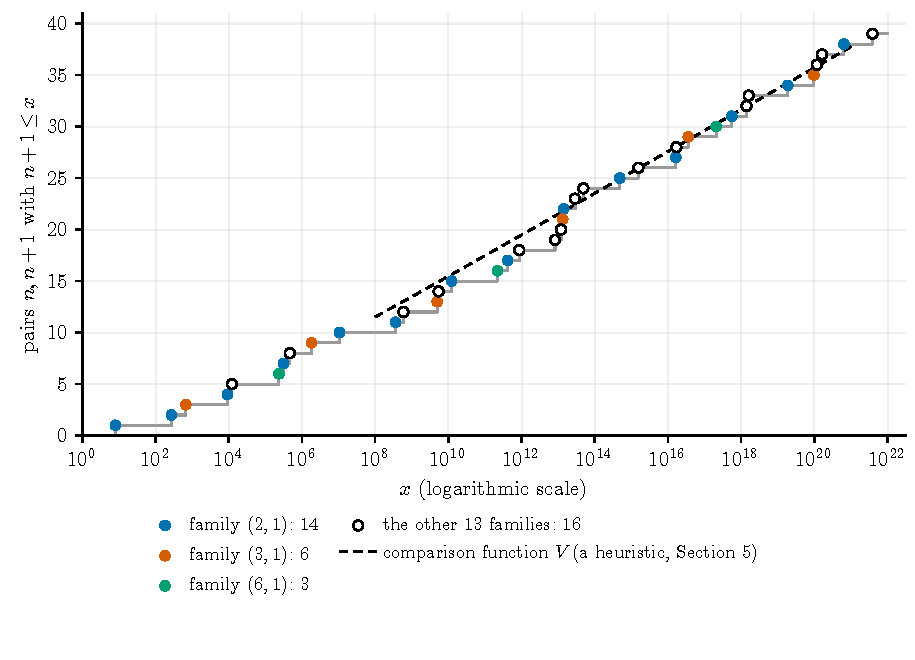
\includegraphics[width=\textwidth]{fig_treppe}
\caption{\textbf{The listed pairs up to $n_0$, and the family each comes from.} The \Z{fampaare} pairs $n, n + 1$ of powerful numbers with
$n \le n_0$ in the list of Proposition~\tref{prop:aufzaehlung}(b), which is complete below $2^{\Z{paare52exp}}$, as a staircase: each step is one pair, and each point is
colored by the family of Section~\tref{sec:familien} that contains it; the families with at least three pairs have their own color. The
positions come from the family formulas of Proposition~\tref{prop:perioden}, and at every power of ten from $10^8$ to $10^{21}$ the
staircase has exactly the number of pairs of our count, of which Table~\ref{tab:modell} shows every second one. The dashed line is the
comparison function of Section~\tref{sec:modell}, a heuristic yardstick, drawn from $10^8$ on, where that table begins.}\label{fig:treppe}
\end{figure}

A positive integer is \emph{powerful} if every prime that divides it divides it at least twice. There are infinitely many $n$ such that
$n$ and $n + 1$ are both powerful; the solutions of Pell equations give them, as Walker recounts \cite[p.~111]{Walker1976}. Erd\H{o}s asked
two further questions \cite{Bloom365}: whether all such pairs come from Pell equations, that is, whether $n$ or $n + 1$ must be a square,
and whether the number $N_1(x)$ of such $n$ with $n + 1 \le x$ is bounded by a power of $\log x$. The first question has a negative answer:
Golomb's pair $12167, 12168$ has no square, and Walker showed that its family is infinite \cite[p.~111]{Walker1976}; Walker also described all
pairs through Pell equations \cite[Sections~2 and~3]{Walker1976}. The second question is open. The best upper bound we know is $N_1(x) \ll x^{29/100 + \epsilon}$,
from a preprint of Reuss \cite[Theorem~4]{Reuss2014}, after $x^{2/5}(\log x)^2$ and $x^{7/19}\log x$ by Chan
\cite[Theorems~3 and~4]{Chan2012} and $x^{\gamma}$ for every $\gamma > 61/180$ by Blomer and Sch{\"o}bel \cite[Theorem~3]{BlomerSchoebel2013}, all three for every fixed distance;
Tao \cite[Corollary~2.11]{Tao2026} proves $x^{2/5 + o(1)}$ for pairs at every fixed distance and discusses the question. The pairs at distance
two, $n - 1$ and $n + 1$ powerful, are the objects of Part~I, where their middles $n$ carry the question of three consecutive powerful
numbers; a question of Golomb about two consecutive odd powerful numbers was answered by Sentance \cite[p.~272]{Sentance1981}.

This part collects what we can prove, compute and measure about the count of pairs, at distance one and at distance two. It establishes an explicit
lower bound of the order $\log x$, with a computed constant, checks the known list of pairs, and places the counting problem for distance two in the kernels that
divide their own $U_1$, of which only \Z{reinhartgerade} with $T_1$ even have been found below $5.325 \cdot 10^{13}$, and which contain the
case in which Tao's argument is weakest, under a squarefreeness assumption.

\paragraph{Main results.}
\begin{itemize}
\item \emph{An explicit lower bound} (Proposition~\tref{prop:csechs}): $\liminf N_1(x)/\log x \ge \Z{csechs}$, from the families of Walker
  with a square and squarefree part at most $\Z{csechsbmax}$, and from those without a square and $bd \le \Z{walkerdmax}$. That there are infinitely many pairs is classical; we did not find an
  explicit constant in the literature.
\item \emph{The count at distance two is a sum over towers} (Proposition~\tref{prop:turmsumme}), and so $P_2(10^h) \ge \Z{turmc}\,h -
  \Z{turmtuerme}$ for every $h$ (Corollary~\tref{cor:untergrenze}). In the box of kernels up to $\Z{kernschranke}$ and middles below
  $10^{\Z{hoehe}}$ the list of pairs at distance two is complete: \Z{zeugenpunkte} with middle divisible by four (Part~I) and \Z{kdpaare}
  with middle $\equiv 2 \pmod 4$ (Proposition~\tref{prop:klassedrei}).
\item \emph{Localization} (Proposition~\tref{prop:lokalisierung}): up to $O(N^{2/9})$, the pairs at distance two with middle at most $N$
  are exactly the first pairs of the kernels $m$ with $m \mid U_1(m)$, so every bound $E_3(N) \ll N^\theta$ on the number of these kernels
  gives $P_2(N) \ll N^{\max(2/9,\,\theta)}$. The case in which the argument of Tao is weakest lies among these kernels when the numbers $n_2$ and $m_2$ of Remark~\tref{rem:tao} are
  squarefree.
\item \emph{The families with a square overtake the comparison function} (Proposition~\tref{prop:transient}): the count of pairs with a square in
  the families with squarefree part up to $\Z{quadbmax}$ exceeds the comparison function of Section~\tref{sec:modell} for every
  $x \ge e^{1000}$, and at every row of the table from $10^{\Z{quadablog}}$ on. So the agreement of such a model with the counts up
  to $n_0$, which we also record, is a fact about that range and not a law.
\end{itemize}

\paragraph{How to read this part.} Every statement is followed by a paragraph \emph{In words} that says what it means with as few formulas as possible; a
reader who wants the results can read the statements and these paragraphs. A reader who wants to check can read the proofs, the paragraphs
\emph{The computation}, and the tables; every number we computed is generated from the data files of the deposit or from a cited constant,
and every numbered statement carries
a label that says whether it is proved, taken from the literature, computed, measured, a heuristic, or open (see the table at the end).
A statement that combines several kinds carries the label of the part that needs the most trust: a proof that uses our own computation is labeled computed, and a proof that uses a published result is labeled proved.
Table~\ref{tab:legende2} collects the notation.

\paragraph{Plan.} Section~\tref{sec:familien} recalls Walker's families and their periods. Section~\tref{sec:aufzaehlung} lists the pairs
up to $2^{\Z{paare52exp}}$ from our own enumeration and checks the published list beyond it inside the families. Section~\tref{sec:schranke}
establishes the lower bound. Section~\tref{sec:modell} sets up the comparison function, marks it as a heuristic, shows that the square families
overtake it, and states the convergence question. Section~\tref{sec:abstandzwei} treats the pairs at distance two: the second class of
middles, the tower sum, the lower bound, the localization and the growth question. Section~\tref{sec:abstandeins} puts the pairs at distance
one on one Pell equation per kernel and tests the third neighbor. Section~\tref{sec:fragen} collects the open questions.

\section{Pell families}\tlabel{sec:familien}

\subsection{Pairs as solutions of one equation}

As in Part~I, $\operatorname{sqfree}(N)$ is the product of the primes that divide $N$ to an odd power, so that
$N = \operatorname{sqfree}(N)\, r^2$ for a positive integer $r$.

\begin{lemma}[powerful numbers]\tlabel{lem:form}\belegart{proved}
A positive integer $n$ is powerful if and only if $n = bY^2$ with $b = \operatorname{sqfree}(n)$ and $b \mid Y$. This is the usual
description of powerful numbers, in the form used below.
\end{lemma}

\begin{proof}
Write $n = bY^2$ with $b = \operatorname{sqfree}(n)$. For a prime $p \mid b$ we have $v_p(n) = 1 + 2v_p(Y)$, which is at least $2$ exactly
when $p \mid Y$. For a prime $p \mid n$ with $p \nmid b$ we have $p \mid Y$ and $v_p(n) = 2v_p(Y) \ge 2$ in any case.
\end{proof}

\inwords Every number is its squarefree part times a square. The number is powerful exactly when the squarefree part divides the
root of the square part; for example $72 = 2 \cdot 6^2$ is powerful because $2 \mid 6$, and $12 = 3 \cdot 2^2$ is not because $3 \nmid 2$.

\begin{proposition}[Walker {\cite[Sections~2 and~3]{Walker1976}}]\tlabel{thm:bijektion}\belegart{literature}
Let $n$ and $n + 1$ be powerful, and put $b = \operatorname{sqfree}(n)$, $d = \operatorname{sqfree}(n + 1)$, $Y^2 = n/b$, $X^2 = (n+1)/d$.
Then
\[
  dX^2 - bY^2 = 1, \qquad b \mid Y, \qquad d \mid X .
\]
Conversely, every solution in positive integers of this equation with $b, d$ squarefree, $b \mid Y$ and $d \mid X$ comes from exactly one
such pair, namely $n = bY^2$.
\end{proposition}

\begin{proof}
The first part is Lemma~\tref{lem:form} applied to $n$ and to $n + 1$. Conversely, $bY^2$ and $dX^2$ are consecutive, and they are
powerful by Lemma~\tref{lem:form}, because $\operatorname{sqfree}(bY^2) = b$ and $\operatorname{sqfree}(dX^2) = d$ for squarefree
$b$ and $d$. The number $n$ determines $b$, $d$, $X$ and $Y$.
\end{proof}

\inwords A pair of consecutive powerful numbers is the same thing as a solution of $dX^2 - bY^2 = 1$ with two divisibility conditions.
Golomb \cite{Golomb1970} sorted the pairs into two types, as Walker recounts in his introduction \cite[p.~111]{Walker1976}, and Walker described both types through
equations of this shape.

We call the set of pairs with a given $(b, d)$ the \emph{family} $(b, d)$. The order matters: in the family $(b, d)$ the smaller number has
squarefree part $b$. As $X^2 - Y^2 = 1$ has no solution in positive integers, $b$ and $d$ are not both $1$. If $b = 1$ or $d = 1$, one of
the two numbers is a square (Walker's type~I); if $b, d \ge 2$, neither is (type~II). By Proposition~\tref{thm:bijektion} every pair lies in
exactly one family.

\subsection{The pairs inside one family}

For type~I with $d = 1$ the equation is Pell's equation $X^2 - bY^2 = 1$. We use the notation of Part~I with $m = b$: $\varepsilon_b =
T_1 + U_1\sqrt{b}$ is its fundamental solution, $\varepsilon_b^{\,k} = T_k + U_k\sqrt{b}$, and $b' = \prod_{p \mid b,\ p \nmid U_1} p$.

\begin{proposition}[Walker {\cite[Theorems 2.2, 2.5, 3.2 and 3.5]{Walker1976}}]\tlabel{prop:perioden}\belegart{literature}
\begin{enumerate}
\item[(i)] Let $b \ge 2$. The pairs of the family $(b, 1)$ are $n = bU_k^{\,2}$, $n + 1 = T_k^{\,2}$ for exactly the $k \ge 1$ with
  $b' \mid k$.
\item[(ii)] Let $d \ge 2$. The family $(1, d)$ needs a solution of $Y^2 - dX^2 = -1$. If there is none, or if $d$ is even, the family is
  empty. Otherwise let $\eta = y_0 + x_0\sqrt{d}$ be the fundamental solution, $\eta^k = Y_k + X_k\sqrt{d}$ for odd $k$, and
  $g = d/\gcd(d, x_0)$. The pairs are $n = Y_k^{\,2}$, $n + 1 = dX_k^{\,2}$ for exactly the odd multiples $k$ of $g$.
\item[(iii)] Let $b, d \ge 2$, and let $\alpha = x_0\sqrt{d} + y_0\sqrt{b}$ be the smallest solution of $dX^2 - bY^2 = 1$ if there is one.
  All solutions are $\alpha^{j} = X\sqrt{d} + Y\sqrt{b}$ with $j$ odd. If $d$ is even and $x_0$ is odd, or $b$ is even and $y_0$ is odd,
  the family is empty. Otherwise its pairs come from exactly the odd multiples $j$ of $\ell$, the product of the odd primes that divide
  $bd$ but not $x_0 y_0$.
\end{enumerate}
\end{proposition}

\begin{proof}
Part~(i) is Lemma~\partref{I}{lem:walker} for $m = b$: $b \mid U_k$ if and only if $b' \mid k$. Part~(ii) follows in the same way. For odd $k$
the binomial theorem gives $X_k = \sum_{i \text{ odd}} \binom{k}{i} y_0^{\,k-i} x_0^{\,i} d^{(i-1)/2} \equiv k\, y_0^{\,k-1} x_0 \pmod p$ for a
prime $p \mid d$, and $y_0^2 \equiv -1 \pmod p$, so $y_0$ is invertible modulo $p$. Hence $p \mid X_k$ if and only if $p \mid k x_0$. If $d$ is
even, then $y_0$ is odd, $dx_0^2 = y_0^2 + 1 \equiv 2 \pmod 8$, so $x_0$ is odd and no $X_k$ with $k$ odd is even. If $d$ is odd, $d \mid X_k$
if and only if $g \mid k$. Part~(iii) is Walker's Theorems 3.2 and 3.5; the description of all solutions as odd powers of $\alpha$ is his
Theorem~3.1, which he takes from \cite[Theorem~9]{Walker1967}.
\end{proof}

\inwords Inside one family the pairs come at regular steps. For the family $(b, 1)$ one takes every $b'$-th power of the Pell solution, for
$(1, d)$ every $2g$-th power starting at the $g$-th, and for type~II the same with $\ell$. We call $b'$, $g$ and $\ell$ the \emph{period} of
the family. Walker proved all three parts; the proof of (i) and (ii) above is short enough to give here.

For the computations we used our own forms of these statements and checked them: part~(i) against direct iteration modulo $b$ for all
\Z{periodepk} squarefree $b \le \Z{periodepkmax}$, and our residue class form of part~(iii) against direct iteration modulo $bd$ for all
\Z{walkerpk} solvable equations with $b, d \ge 2$ and $bd \le \Z{walkerpkmax}$; all agreed. For the families in
Table~\ref{tab:familien} we also computed $b'$, $g$ and $\ell$ from Walker's definitions and found the periods of our computation.

\inwords The formulas were not only cited: a computer followed the powers one by one and found the pairs exactly where the formulas for parts (i) and (iii) say.

\subsection{The families of the known pairs}

Each family grows geometrically. Here and below, $\log$ is the natural logarithm; Table~\ref{tab:familien} gives
$\log_{10}$ for readability. If $n_1$ is its first pair, the $j$-th is about $n_1 F^{\,j-1}$, where $\log F = 2b'\log\varepsilon_b$ for
the family $(b, 1)$, $\log F = 4g\log\eta$ for $(1, d)$, and $\log F = 4\ell\log\alpha$ for type~II. Throughout this part
$n_0 = \Z{paarletzt}$ is term number \Z{fampaare} of the list in Section~\tref{sec:aufzaehlung}, so
$n_0 \approx \Z{paargrenze}$.
Table~\ref{tab:familien} lists the families of the \Z{fampaare} pairs of that list with $n \le n_0$: \Z{famzahl} families,
\Z{famquadrat} pairs with a square and \Z{famohne} without. The first pairs of the families $(46, 1)$, $(6, 1)$, $(1, 5)$ and $(3, 7)$ are the four examples in Walker's paper
\cite[pp.~113 and~116]{Walker1976}.

\begin{table}[ht]
\centering
\begin{tabular}{crrrr}
\hline
family $(b, d)$ & period & $\log_{10} n_1$ & $\log_{10} F$ & pairs \\
\hline
\Z{famtab}
\hline
\end{tabular}
\caption{The families of the pairs $n, n+1$ of powerful numbers with $n \le n_0 \approx \Z{paargrenze}$, ordered by their first pair $n_1$. The
period is $b'$, $g$ or $\ell$ of Proposition~\tref{prop:perioden}; $F$ is the growth factor from one pair of the family to the next.
Each row is checked against three computations: the count in the list of pairs, the count predicted from the family, and, for type~II,
the pairs generated from the family and factored.}\label{tab:familien}
\end{table}

\inwords Most of the known pairs sit in a few families. The family $(2, 1)$, which starts with $8$ and $9$, alone has \Z{famtabzwei} of them,
because its growth factor is small. Most other families contribute a single pair so far.

\subsection{Notation and terms at a glance}\tlabel{sec:legende}

Table~\ref{tab:legende2} collects the symbols and words of this part, with the place where each is defined.

\begin{table}[tp]
\centering
\footnotesize
\begin{tabular}{p{3.0cm} p{7.6cm} l}
\hline
symbol or term & meaning & defined in \\
\hline
powerful & every prime factor occurs at least twice & Lemma~\tref{lem:form} \\
$\operatorname{sqfree}(N)$ & the product of the primes that divide $N$ to an odd power & \S\tref{sec:familien} \\
family $(b, d)$ & the pairs $n, n + 1$ with $\operatorname{sqfree}(n) = b$ and $\operatorname{sqfree}(n + 1) = d$ & \S\tref{sec:familien} \\
type I, type II & one of $n$, $n + 1$ is a square ($b = 1$ or $d = 1$); neither is ($b, d \ge 2$) & \S\tref{sec:familien} \\
$\varepsilon_b$, $T_k$, $U_k$, $b'$ & as in Part~I, with the kernel $m = b$ & Proposition~\tref{prop:perioden} \\
$\eta$, $g$ & the smallest solution $y_0 + x_0\sqrt{d}$ of $y^2 - dx^2 = -1$, and $g = d/\gcd(d, x_0)$ & Proposition~\tref{prop:perioden} \\
$\alpha$, $\ell$ & the smallest solution $x_0\sqrt{d} + y_0\sqrt{b}$ of $dX^2 - bY^2 = 1$, and the product of the odd primes of $bd$
  that do not divide $x_0 y_0$ & Proposition~\tref{prop:perioden} \\
period & $b'$, $g$ or $\ell$: the step between the powers that give pairs & Proposition~\tref{prop:perioden} \\
growth factor $F$ & the factor from one pair of a family to the next; $\log F = 2b'\log\varepsilon_b$, $4g\log\eta$ or $4\ell\log\alpha$
  & \S\tref{sec:familien} \\
$n_0$ & term number \Z{fampaare} of the list of Section~\tref{sec:aufzaehlung}; the range of Table~\ref{tab:familien} is $n \le n_0$
  & \S\tref{sec:familien} \\
$N_1(x)$ & the number of pairs with $n + 1 \le x$ & Proposition~\tref{prop:csechs} \\
pair at distance two, middle & powerful numbers $n - 1$, $n + 1$; the number $n$ between them & \S\tref{sec:abstandzwei} \\
kernel $m$, $m'$, lattice point & as in Part~I: $m = \operatorname{sqfree}(n^2 - 1)$, and $n = T_k(m)$ with $k$ an odd multiple of $m'$
  & Lemma~\partref{I}{lem:gerademitte} \\
$P_2(N)$, $P_2(N; M)$ & the number of middles $n \le N$, all of them or those with kernel at most $M$ & \S\tref{sec:abstandzwei} \\
discard criterion & a proved lower bound for $T_k(m)$ that removes a kernel before any $T_k$ is computed & Theorem~\partref{I}{thm:reduktion} \\
tower & the middles $T_k(m)$ of one kernel $m$ with $T_1(m)$ even, one for each odd multiple $k$ of $m'$ & \S\tref{sec:abstandzwei} \\
$w(m)$, $c_M$ & the rate $1/(2m'\log_{10}\varepsilon_m)$ of one tower in pairs per decimal digit, and the sum of these rates up to $M$
  & Proposition~\tref{prop:turmsumme} \\
$E_J(N)$ & the number of kernels with $m' < J$ and $T_1(m)$ even whose first middle is at most $N$ & Proposition~\tref{prop:lokalisierung} \\
index $m'$, wing (ii), rung & the product of the primes of $m$ that do not divide $U_1$; the kernels with $m \mid U_1$; one pair of a tower
  & Part~I \\
$v_p(N)$, $c_1$, $c_2$, $a_p$ & the exponent of $p$ in $N$; the constants of $Q(x)$; the proportion of $n$ with $v_p(n) = 1$
  & \S\tref{sec:modell} \\
$N_Q^{*}(L)$ & the count of the pairs with a square from the family periods, by the floor formula & Proposition~\tref{prop:transient} \\
$Q(x)$, $\rho(x)$ & the number of powerful numbers up to $x$, and the derivative of its two main terms & \S\tref{sec:modell} \\
$C$, $V(x)$ & the local correction factor and the comparison function, a heuristic yardstick & Definition~\tref{def:vergleich} \\
$N_Q(x)$, born & the pairs with a square in the families with $b, d \le \Z{quadbmax}$; a family is born at the logarithm of its first pair
  & Proposition~\tref{prop:transient} \\
$D$, $R$, third number & $D = \operatorname{sqfree}(a(a + 1))$, $a(a + 1) = DR^2$; the neighbor $a - 1$ or $a + 2$ that is not excluded by $2$
  & Proposition~\tref{prop:abstandeins} \\
\hline
\end{tabular}
\caption{Symbols and terms of Part II.}\label{tab:legende2}
\end{table}

\section{Enumeration}\tlabel{sec:aufzaehlung}

\begin{proposition}[the known pairs]\tlabel{prop:aufzaehlung}\belegart{computed}
\begin{enumerate}
\item[(a)] There are exactly \Z{paare52} pairs $n, n+1$ of powerful numbers with $n + 1 \le 2^{\Z{paare52exp}}$.
\item[(b)] Let $n_0$ be term number \Z{fampaare} of the b-file of OEIS A060355 \cite{OEISA060355}, computed by D.~Johnson, which lists
  such pairs by their smaller member $n$. The families of Section~\tref{sec:familien}, with a square and squarefree part at most
  $\Z{csechsbmax}$ or without a square and $bd \le \Z{walkerdmax}$, generate exactly \Z{fampaare} pairs with $n \le n_0$ from their
  fundamental solutions, each checked by complete factorization and by the identity $dX^2 - bY^2 = 1$ with $b \mid Y$ and $d \mid X$. The
  first \Z{paare52} of them are the pairs in (a), and the \Z{fampaare} pairs are exactly the first \Z{fampaare} terms of the b-file
  (Proposition~\tref{prop:quadratvollstaendig}). That no pair with $n \le n_0$ lies outside these families is a statement of that
  enumeration, not of ours.
\end{enumerate}
\end{proposition}

\begin{proof}[The computation]
(a) We listed all powerful numbers below $2^{\Z{paare52exp}}$ block by block, the block $k$ being $[2^k, 2^{k+1})$, each number written as
$a^2 b^3$ with $b$ squarefree; this form is unique. The size of every block agrees with the count $\sum_{b} \lfloor \sqrt{x/b^3} \rfloor$ over
squarefree $b$, taken at the two ends of the block. Inside a block the pairs are neighbors at distance one. A pair across two blocks would be
$(2^k - 1, 2^k)$, and $2^k - 1$ is not powerful for $2 \le k \le \Z{mersennemax}$, by complete factorization.
(b) The pairs are generated by the recursion of the Pell equation from the fundamental solution of each family, as in the proof of
Proposition~\tref{prop:quadratvollstaendig}; both members of every pair are factored completely, and the identity is checked with the
squarefree parts $b$ and $d$. The comparison with the b-file is made at run time against a copy that the reader supplies; the terms of the
b-file are not stored in the data deposit.
\end{proof}

\inwords Up to $2^{\Z{paare52exp}}$ we found all pairs ourselves. Beyond that we used a published list and
checked that each of its entries really is a pair; we did not check that the list misses nothing.

Mian and Siddique \cite{MianSiddique2026} describe the larger enumerations as exhaustive below $10^{22}$ but not certified. We rely on
it only where we say so. The next statement checks it inside the families of Section~\tref{sec:familien}, independently of the list.

\begin{proposition}[completeness inside the families]\tlabel{prop:quadratvollstaendig}\belegart{computed}
\begin{enumerate}
\item[(a)] In the families with a square, $(b, 1)$ and $(1, d)$ with $b, d \le \Z{quadratbmax}$, the pairs with $n \le n_0$ are exactly
  the \Z{famquadrat} pairs with a square among the terms of Proposition~\tref{prop:aufzaehlung}(b). They lie in \Z{famquadratfam} families.
\item[(b)] In the families without a square with $bd \le \Z{walkerdmax}$, the pairs with $n \le n_0$ are exactly the \Z{famohne} pairs
  without a square among those terms.
\end{enumerate}
\end{proposition}

\begin{proof}[The computation]
For every family in the range we generated its pairs from Proposition~\tref{prop:perioden} up to $n_0$ and compared them with the terms, in
both directions: no generated pair is missing from the terms, and no term with a square (in (a)) or without a square (in (b)) is missing
from the generated pairs. For (b) each generated pair was also factored completely, and both numbers are powerful.
\end{proof}

\inwords Every one of the \Z{fampaare} known pairs comes out of our own family computation, and within the families we searched our
computation finds no pair that the list lacks. So the list is complete for these families. Outside them, for example a family $(b, 1)$ with
$b > \Z{quadratbmax}$ whose first pair lies below $n_0$, a missing pair would not be noticed here.

\section{An explicit lower bound}\tlabel{sec:schranke}

\begin{proposition}[explicit lower bound]\tlabel{prop:csechs}\belegart{computed}
Let $N_1(x)$ count the pairs $n, n+1$ of powerful numbers with $n + 1 \le x$. Then
\[
  \liminf_{x\to\infty} \frac{N_1(x)}{\log x} \ge \Z{csechs} .
\]
The \Z{csechsfamq} nonempty families with a square and squarefree part at most $\Z{csechsbmax}$ contribute \Z{csechsquadrat}, and the
\Z{csechsfamw} nonempty families without a square and with $bd \le \Z{walkerdmax}$ contribute \Z{csechswalker}.
\end{proposition}

\begin{proof}
Let $F$ be the growth factor of a nonempty family, as in Section~\tref{sec:familien}. We first show that its $j$-th pair satisfies
$n_j + 1 \le F^{\,j}$. In the family $(b, 1)$ the $j$-th pair has $n_j + 1 = T_{jb'}^{\,2}$ by Proposition~\tref{prop:perioden}(i), and
$T_k = (\varepsilon_b^{\,k} + \varepsilon_b^{-k})/2 \le \varepsilon_b^{\,k}$, so $n_j + 1 \le \varepsilon_b^{\,2jb'} = F^{\,j}$. In the family
$(1, d)$ the $j$-th pair comes from $k = (2j - 1)g$, and for odd $k$ the conjugate of $\eta^k$ is $-\eta^{-k}$, so
$X_k\sqrt{d} = (\eta^k + \eta^{-k})/2 \le \eta^k$ and $n_j + 1 = dX_k^{\,2} \le \eta^{2(2j-1)g} \le \eta^{4jg} = F^{\,j}$. For type~II the $j$-th
pair comes from the exponent $(2j - 1)\ell$, the conjugate of $\alpha^i = X\sqrt{d} + Y\sqrt{b}$ is $X\sqrt{d} - Y\sqrt{b} = \alpha^{-i}$, and
the same computation gives $n_j + 1 = dX^2 \le \alpha^{4j\ell} = F^{\,j}$.

Hence a family has at least $\lfloor \log x / \log F \rfloor \ge \log x / \log F - 1$ pairs with $n + 1 \le x$. Different families have
different pairs by Proposition~\tref{thm:bijektion}. So for every finite set $S$ of nonempty families
\[
  N_1(x) \ge \sum_{f \in S} \Bigl( \frac{\log x}{\log F_f} - 1 \Bigr), \qquad
  \liminf_{x\to\infty} \frac{N_1(x)}{\log x} \ge \sum_{f \in S} \frac{1}{\log F_f} .
\]
For the two sets named in the statement we computed the sums; the total is rounded down.
\end{proof}

\inwords Each family on its own produces pairs at a steady rate on a logarithmic scale: the number of its pairs below $x$ grows like
$\log x$ divided by the logarithm of its growth factor. Since no pair belongs to two families, the rates add up. Adding them for all
families up to the stated sizes gives the constant. Families outside these ranges can only increase it.

\section{A heuristic comparison model, and the convergence question}\tlabel{sec:modell}

This section compares the count $N_1(x)$ of Section~\tref{sec:schranke} with a function that a simple probabilistic picture suggests. The
picture is a heuristic. We use the function only as a yardstick, and we do not claim that it predicts anything; the only statement of
this section that is not a heuristic is Proposition~\tref{prop:transient}, and the lower bound of Section~\tref{sec:schranke} does not depend on the picture.

\subsection{The comparison function}

Let $Q(x)$ be the number of powerful numbers up to $x$. Erd\H{o}s and Szekeres found the main term, and Bateman and Grosswald proved
$Q(x) = c_1 \sqrt{x} + c_2 x^{1/3} + O(x^{1/6})$ \cite{ErdosSzekeres1934}, \cite[Theorem~1]{BatemanGrosswald1958}, with $c_1 = \zeta(3/2)/\zeta(3)$ and $c_2 = \zeta(2/3)/\zeta(2)$, so that $c_2 < 0$. Let
$\rho(x) = c_1/(2\sqrt{x}) + c_2/(3x^{2/3})$ be the derivative of the two main terms.

\begin{definition}[comparison function; a heuristic]\tlabel{def:vergleich}\belegart{heuristic}
For a prime $p$ let $a_p = (p - 1)/p^2$, the proportion of integers $n$ with $v_p(n) = 1$, and let
\[
  C = \prod_{p} \frac{1 - 2a_p}{(1 - a_p)^2}, \qquad V(x) = C \int_8^x \rho(t)^2\, dt .
\]
\end{definition}

The picture behind $V$ is this. If ``$n$ is powerful'' and ``$n + 1$ is powerful'' were independent events of probability $\rho(n)$ each, the
expected number of pairs with $n + 1 \le x$ would be about $\int_8^x \rho(t)^2\, dt$, which grows like $(c_1^2/4) \log x = \Z{naivrate} \log x$.
The events are not independent: a prime $p$ cannot divide both $n$ and $n + 1$, so the events $v_p(n) = 1$ and $v_p(n + 1) = 1$ exclude
each other. Under the picture, the proportion of $n$ with $v_p(n) \ne 1$ and $v_p(n + 1) \ne 1$ is $1 - 2a_p$ instead of $(1 - a_p)^2$, and
the factor $C$ collects this correction over all primes, in the manner of the Hardy--Littlewood constants. Two assumptions enter here and
are not derived: that the primes act independently, and that these proportions, which are densities over all integers, may be applied to
powerful numbers; among powerful numbers the share of $n$ with $4 \mid n$ has a different limit (Remark~\partref{I}{rem:anteil}).
Numerically $C = \Z{modellc}$, so
$V(x)$ grows like $\Z{modellrate} \log x$. Heuristics with a local factor at each prime are used for related counting problems, for example
in \cite{vanDoorn2026}.

\inwords Powerful numbers get rarer as they grow, at a known rate. If two neighbors were powerful independently of each other, one could
compute how many pairs to expect. They are not independent, because a prime never divides two neighbors at once, and $C$ is one simple
correction for that, not a derived one. The result is a curve to compare with, not a prediction.

Table~\ref{tab:modell} sets $V$ against the count. Up to $n_0$ the list has \Z{modellnull} pairs; it is complete below $2^{\Z{paare52exp}}$
and inside the families of Proposition~\tref{prop:quadratvollstaendig}, and beyond that it is described as exhaustive but not certified
\cite{MianSiddique2026}. The comparison function gives \Z{modellnullkorr}, and the independent picture gives \Z{modellnullnaiv}. The
constant $C$ and the function $\rho$ contain nothing fitted to the data: we computed $V$ before we compared it with the terms beyond
$2^{\Z{paare52exp}}$, where the count is \Z{modellneu} against \Z{modellneukorr} for $V$ and \Z{modellneunaiv} for the independent picture.
The agreement is a fact about this range, within a scatter of about $\sqrt{N}$ for a count of $N$ pairs; beyond $2^{\Z{paare52exp}}$ the
comparison does not separate $V$ from the independent picture. The next statement shows that the agreement does not last.

\begin{table}[ht]
\centering
\small
\begin{tabular}{rrrr}
\hline
$\log_{10} x$ & pairs counted & $V(x)$ & independent picture \\
\hline
\Z{modelltab}
\hline
\end{tabular}
\caption{The number of pairs $n, n + 1$ with $n + 1 \le x$, the comparison function $V(x)$ of Definition~\tref{def:vergleich}, and the
uncorrected integral $\int_8^x \rho^2$. The counts up to $2^{\Z{paare52exp}}$ are our own enumeration; beyond it they come from the terms of
Proposition~\tref{prop:aufzaehlung}(b).}\label{tab:modell}
\end{table}

\subsection{The families with a square overtake the comparison function}

Let $N_Q(x)$ be the number of pairs $n, n + 1$ with $n + 1 \le x$ that lie in a family $(b, 1)$ or $(1, d)$ with $b, d \le \Z{quadbmax}$. By
Proposition~\tref{prop:perioden} these families are known exactly. For a family $f$ with first pair $n_1$ and growth factor $F$ put
$t_f = \log n_1$; we say the family is \emph{born} at $\log x = t_f$. By the formulas of Section~\tref{sec:familien}, $n_j + 1$ is
$(\alpha^{k} + \alpha^{-k})^2/4$ times a constant, with $\alpha$ the unit of the family and $k$ growing by the period from one pair to the
next; so $\log(n_j + 1) = \log(n_1 + 1) + (j - 1) \log F - \delta_j$ with $0 \le \delta_j < 2\log 2$, the correction coming from the
decreasing terms $\alpha^{-k}$. The count
\[
  N_Q^{*}(L) = \sum_{f} \max\Bigl(0,\ \Bigl\lfloor \frac{L - t_f}{\log F_f} \Bigr\rfloor + 1\Bigr),
\]
over the families with $b, d \le \Z{quadbmax}$, therefore agrees with $N_Q(e^L)$ except that a pair within $1/n_1$ of the boundary on the
logarithmic scale may fall on the wrong side.

\begin{proposition}[the families with a square overtake the comparison function]\tlabel{prop:transient}\belegart{computed}
\begin{enumerate}
\item[(a)] Table~\ref{tab:quad} gives $N_Q^{*}(L)$ and $V(e^L)$ for \Z{quadzeilen} values of $L = \log x$ up to $1000$. On a finer grid
  than the table, $N_Q^{*}$ first exceeds $V$ at $L = \Z{quadkreuz}$, that is, at $x \approx 10^{\Z{quadkreuzlog}}$; at the next row of the
  table it is below $V$ again, and from $L = \Z{quadab}$ on it is above $V$ at every row of the table.
\item[(b)] For every $L \ge 1000$, $N_Q(e^L) > V(e^L)$.
\end{enumerate}
\end{proposition}

\begin{table}[ht]
\centering
\small
\begin{tabular}{rrrrr}
\hline
$L = \log x$ & $N_Q^{*}(L)$ & $V(e^L)$ & independent picture & rate of the families born \\
\hline
\Z{quadtab}
\hline
\end{tabular}
\caption{The pairs with a square in the families with $b, d \le \Z{quadbmax}$, counted exactly from the family periods, against the
comparison function. The last column is $\sum 1/\log F$ over the families born by $L$, the rate at which $N_Q$ grows there.}\label{tab:quad}
\end{table}

\begin{proof}
(a) is the computation of the table. (b) Let $\mathcal{F}$ be the set of the \Z{quadgeboren} families with $b, d \le \Z{quadbmax}$ that are
born by $L = 1000$, and let $s = \sum_{f \in \mathcal{F}} 1/\log F_f = \Z{quadrate1000}$. Write $y_f(L) = (L - t_f)/\log F_f$. The $j$-th
pair of $f$ has $\log(n_j + 1) \le L$ as soon as $\log(n_1 + 1) + (j - 1) \log F_f \le L$, that is, $j \le (L - \log(n_1 + 1))/\log F_f + 1$; so
$f$ has more than $(L - \log(n_1 + 1))/\log F_f \ge y_f(L) - 1/(n_1 \log F_f)$ pairs with $n + 1 \le e^L$, and the last term is below $0.05$,
because $n_1 \ge 8$ and $\log F_f \ge 2 \log(2 + \sqrt 3) > 2.6$ for every family. On the other hand, each term of $N_Q^{*}(1000)$ is at most
$y_f(1000) + 1$. So for $L \ge 1000$,
\[
  N_Q(e^L) \;>\; \sum_{f \in \mathcal{F}} y_f(L) - 0.05\,|\mathcal{F}| \;\ge\; \bigl(N_Q^{*}(1000) - |\mathcal{F}|\bigr) - 0.05\,|\mathcal{F}|
  + s\,(L - 1000)\]
and $0.05\,|\mathcal{F}| < \Z{quadslack}$, so
\[
  N_Q(e^L) \;>\; \Z{quadrest1000} - \Z{quadslack} + s\,(L - 1000) .
\]
On the other side, $\frac{d}{dL} V(e^L) = C \rho(e^L)^2 e^L = C \bigl(c_1/2 + (c_2/3) e^{-L/6}\bigr)^2 < C c_1^2/4 = \Z{modellrate}$, because
$c_2 < 0$. Hence $V(e^L) \le V(e^{1000}) + \Z{modellrate}\,(L - 1000)$ with $V(e^{1000}) = \Z{quadv1000}$. Since $\Z{quadrest1000} - \Z{quadslack} >
\Z{quadv1000}$ and $s > \Z{modellrate}$, the claim follows. The value of $V(e^{1000})$ is rounded to one decimal and the product $C$ is
truncated; truncating $C$ increases $V$, and the margin is larger than the rounding, so both errors are on the safe side.
\end{proof}

\inwords The comparison curve grows at a fixed rate on a logarithmic scale. The families with a square alone grow faster once enough of
them have been born, and from $10^{\Z{quadablog}}$ on, at every row of the table, they produce more pairs than the curve gives for all pairs
together; for all $x \ge e^{1000}$ this is proved. So the curve matches the counts only in the range we can see, and it must fail beyond it.
It is a yardstick for the present, not a law.

\subsection{The convergence question}

By Proposition~\tref{prop:csechs}, $\liminf N_1(x)/\log x$ is at least the sum of $1/\log F$ over any finite set of families. The sum over the
families with a square and squarefree part at most $B$ is \Z{teilsumq1} for $B = 10$ and \Z{teilsumq2} for $B = 100$; Table~\ref{tab:teilsum} continues it and
adds the families without a square with $bd \le B$.

\begin{table}[ht]
\centering
\small
\begin{tabular}{rrrr}
\hline
$\log_{10} B$ & with a square, squarefree part $\le B$ & without a square, $bd \le B$ & sum \\
\hline
\Z{teilsumtab}
\hline
\end{tabular}
\caption{The partial sums $\sum 1/\log F$ over the families of Section~\tref{sec:familien}. The last entry of the last column is the constant
of Proposition~\tref{prop:csechs}.}\label{tab:teilsum}
\end{table}

\begin{question}[convergence of the rates]\tlabel{q:konvergenz}\belegart{open}
Does $\sum_f 1/\log F_f$, taken over all families, converge?
\end{question}

The increase per decade of $B$ shrinks in both columns of the table. We counted where the last increase comes from: in the decade
$10^5 < B \le 10^6$, families with $\log \varepsilon \le 100$ supply \Z{zuwq}\,\% of it among the families with a square and \Z{zuww}\,\%
among those without, and the largest one percent of the families supply \Z{zuwtopq}\,\% and \Z{zuwtopw}\,\%. So in the last decade we
computed, the increase is carried by a small share of the families, those with small units, not by many small contributions. Whether this
continues is not known.

A positive answer would not by itself give an asymptotic formula for $N_1(x)$. Families keep being born, and each newborn family adds a
pair at once; turning the sum of the rates into the rate of $N_1(x)$ needs control of how many families are born below every height, which we
do not have. The towers of Section~\tref{sec:abstandzwei} pose the same question for distance two, as Question~\tref{q:wachstum}.

This is also where an answer to the second question of Erd\H{o}s could come from. Every pair belongs to exactly one family, and a family has
about $\log x/\log F$ pairs below $x$. So $N_1(x)$ is governed by two quantities: how many families are born below $x$, and the sum of
their rates, which is Question~\tref{q:konvergenz}. If the number of families born below $x$ were bounded by a power of $\log x$, so would
be $N_1(x)$, and the answer to the question of Erd\H{o}s would be yes. We know no such bound, and no bound for the number of families
better than the upper bounds for $N_1(x)$ itself recalled in the introduction. We do not know whether it holds.

\inwords Every family contributes a rate, and the rates add up. Whether the total of all rates is finite is open. Our partial sums grow
more and more slowly, but they are driven by a small share of the families, those with small units, so a few more decades would not settle it.
Erd\H{o}s's question would be answered by showing that new families are born rarely enough; we cannot show this.

\section{Pairs at distance two}\tlabel{sec:abstandzwei}

A \emph{pair at distance two} is a pair $n - 1$, $n + 1$ of powerful numbers, and $n$ is its \emph{middle}. By
Lemma~\partref{I}{lem:gerademitte} the middle is even, and $n = T_k(m)$ for exactly one squarefree odd $m \ge 3$ with $T_1(m)$ even and one
odd multiple $k$ of $m'$. The kernel satisfies $m \equiv 7 \pmod 8$ when $4 \mid n$, and $m \equiv 3 \pmod 8$ when $n \equiv 2 \pmod 4$. We
write
\[
  P_2(N) = \#\{\, n \le N : n - 1 \text{ and } n + 1 \text{ are powerful} \,\},
\]
and $P_2(N; M)$ for the same count restricted to kernels $m \le M$. Proposition~\partref{I}{prop:paarliste} lists the middles divisible by
four in a box. The next statement does the same for the other middles, and the rest of the section counts both. Figure~\ref{fig:turmwald}
shows all these pairs at once.

\begin{figure}[t]
\centering
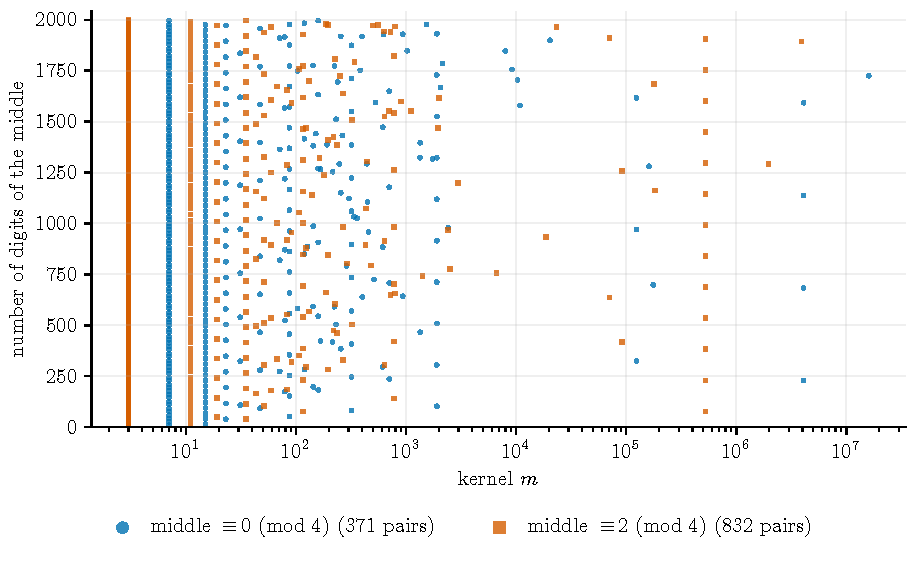
\includegraphics[width=\textwidth]{fig_turmwald}
\caption{\textbf{The pairs at distance two stand in towers.} The pairs at distance two with middle below $10^{\Z{hoehe}}$ and kernel at most $\Z{kernschranke}$, each placed at its kernel $m$
and the number of digits of its middle. The pairs of one kernel stand in a column at equal distances, the towers of
Proposition~\tref{prop:turmsumme}. The kernel $m = 3$ alone gives \Z{kddrei} of them. The column at $m = \Z{einkernm}$, with $m' = 3$, is
the kernel from the discussion of Question~\tref{q:wachstum}.}\label{fig:turmwald}
\end{figure}

\subsection{The middles that are not divisible by four}

\begin{proposition}[the middles that are not divisible by four]\tlabel{prop:klassedrei}\belegart{computed}
\begin{enumerate}
\item[(a)] Among the \Z{kdkerne} squarefree $m \equiv 3 \pmod 8$ with $m \le \Z{kdschranke}$, exactly \Z{kdkandidaten} pass the discard
  criterion of Theorem~\partref{I}{thm:reduktion} for the height $10^{\Z{hoehe}}$; the largest of them is $\Z{kdkernmax}$. Their lattice points
  $(m, k)$ with $T_k(m) < 10^{\Z{hoehe}}$ number \Z{kdpunkte}. For \Z{kdungerade} of them $T_1(m)$ is odd, and the other \Z{kdpaare} are
  exactly the middles $n \equiv 2 \pmod 4$ of pairs at distance two with $n < 10^{\Z{hoehe}}$ and $\operatorname{sqfree}(n^2 - 1) \le
  \Z{kdschranke}$.
\item[(b)] These \Z{kdpaare} middles have \Z{kdpaarkerne} different kernels, and the kernel $m = 3$ alone gives \Z{kddrei} of them.
\item[(c)] The list in (a) contains every middle $n \equiv 2 \pmod 4$ with $n < \Z{ohnetripelsicher}$, every such middle with
  $n < \Z{ohnetripel}$ if Reinhart's extended search missed nothing (Remark~\partref{I}{rem:reinhartliste}), and every such middle with
  $n < 10^{\Z{vollexpo}}/27$ whose kernel does not divide $U_1$.
\end{enumerate}
\end{proposition}

\begin{proof}
(a) is the computation of Theorem~\partref{I}{thm:reduktion}, run with the residue class $3$ in place of $7$, together with
Lemma~\partref{I}{lem:gerademitte}: a lattice point with $T_1$ odd has $T_k$ odd and gives no pair. (b) is a count in the list of (a).
(c) Let $n$ be such a middle and $m$ its kernel. Remark~\partref{I}{rem:siebenundzwanzig} gives the bound $T_k \ge (m^{3/2}/m')^{m'}$ in this
class too, so the proof of Corollary~\partref{I}{cor:kern} applies: if $m \nmid U_1$, then $m^{4.5}/27 < n$, and $m < \Z{kdschranke}$ for
$n < 10^{\Z{vollexpo}}/27$. If $m \mid U_1$, then $m^{3/2} < T_1(m) \le n$, so $n < \Z{ohnetripelsicher}$ forces $m < 1.5 \cdot 10^{12}$, the
range in which Reinhart's list of such kernels is complete \cite[Remark~5.5]{Reinhart2023}, and $n < \Z{ohnetripel}$ forces
$m < 5.325 \cdot 10^{13}$, the range of his extended search \cite{Reinhart2024}. The list has two kernels $m \equiv 3 \pmod 8$,
$1\,752\,299$ below the smaller bound and $20\,256\,129\,307\,923$ below the larger one. The first lies in the box of (a); its $T_1$ has
\Z{kdreinhartungst} digits and is odd. For the second, $T_1$ is even and has \Z{kdreinhartst} digits, so its first middle is far above
$\Z{ohnetripel}$.
\end{proof}

\inwords The middles of the form $4j + 2$ come from the kernels $m$ of the form $8j + 3$. In the box of kernels up to $\Z{kdschranke}$ and
middles below $10^{\Z{hoehe}}$ there are \Z{kdpaare} of them, and most come from a single kernel, $m = 3$. None of them is the middle of a
triple, since such a middle is divisible by $2$ exactly once.

\subsection{The count is a sum over towers}

For a kernel $m$ with $T_1(m)$ even, the middles $T_k(m)$ with $k$ an odd multiple of $m'$ form the \emph{tower} over $m$.

\begin{proposition}[the count is a sum over towers]\tlabel{prop:turmsumme}\belegart{proved}
For all integers $N, M \ge 1$,
\[
  P_2(N; M) \;=\; \sum_{\substack{3 \le m \le M \text{ odd, squarefree}\\ T_1(m) \text{ even}}}
  \#\bigl\{\, k \text{ an odd multiple of } m' : k \log \varepsilon_m \le \log (2N) \,\bigr\} .
\]
\end{proposition}

\begin{proof}
By Lemma~\partref{I}{lem:gerademitte} the middles $n \le N$ with kernel $m \le M$ correspond one to one to the pairs $(m, k)$ in the sum with
$T_k(m) \le N$. It remains to show that $T_k \le N$ exactly when $\varepsilon_m^{\,k} \le 2N$. We have $2T_k = \varepsilon_m^{\,k} +
\varepsilon_m^{-k}$ with $0 < \varepsilon_m^{-k} < 1$. If $T_k \le N$, then $\varepsilon_m^{\,k} < 2T_k \le 2N$. If $\varepsilon_m^{\,k} \le 2N$,
then $2T_k < 2N + 1$, and since $2T_k$ is an integer, $2T_k \le 2N$.
\end{proof}

\inwords Each kernel carries a tower of pairs, one on every rung $k$, and the rungs are evenly spaced on a logarithmic scale: from one rung to
the next the middle grows by the factor $\varepsilon_m^{\,2m'}$. Counting the pairs below a height is counting rungs below that height, tower by
tower.

We evaluated the right side for the kernels that pass the discard criterion in both classes and compared it with the lattice points that the
searches of Theorem~\partref{I}{thm:reduktion} and Proposition~\tref{prop:klassedrei} found. Table~\ref{tab:turm} shows six heights; the two
agree at every height in both classes. The last two columns are a negative control: the same count with the step $\log T_1$ in place of
$\log \varepsilon_m$, an error of an early version of our program, gives larger counts, which are wrong.

\begin{table}[ht]
\centering
\small
\begin{tabular}{rrrrr}
\hline
 & \multicolumn{2}{c}{pairs, counted and by the tower sum} & \multicolumn{2}{c}{negative control (step $\log T_1$)} \\
$h$ & middle $\equiv 0 \pmod 4$ & middle $\equiv 2 \pmod 4$ & middle $\equiv 0 \pmod 4$ & middle $\equiv 2 \pmod 4$ \\
\hline
\Z{turmtab}
\hline
\end{tabular}
\caption{Pairs at distance two with middle at most $10^h$ and kernel at most $\Z{kernschranke}$. The counted pairs and the tower sum of
Proposition~\tref{prop:turmsumme} agree in every row.}\label{tab:turm}
\end{table}

Each tower adds one pair every time $\log_{10} N$ grows by $2m' \log_{10} \varepsilon_m$. So $P_2(10^h; M)$ grows with $h$ at the average rate
\[
  c_M = \sum_{\substack{3 \le m \le M \text{ odd, squarefree}\\ T_1(m) \text{ even}}} w(m), \qquad w(m) = \frac{1}{2m' \log_{10} \varepsilon_m},
\]
pairs per decimal digit. For the towers of Table~\ref{tab:turm} the rate is \Z{turmc7} for the middles divisible by four and \Z{turmc3} for the
others. This rate belongs to the kernels up to $M$; it is not a rate for $P_2$ itself, because kernels above $M$ add towers of their own.
Whether $c_M$ stays bounded as $M$ grows is Question~\tref{q:wachstum}.

\begin{corollary}[lower bound at every height]\tlabel{cor:untergrenze}\belegart{computed}
For every integer $h \ge 1$,
\[
  P_2(10^h) \;\ge\; \Z{turmc}\, h - \Z{turmtuerme} .
\]
For the middles divisible by four alone, the count is at least $\Z{turmc7}\, h - \Z{turmtuerme7}$.
\end{corollary}

\begin{proof}
Take the \Z{turmtuerme} kernels $m \le \Z{kernschranke}$ with $T_1(m)$ even that pass the discard criterion, \Z{turmtuerme7} of them with
$m \equiv 7 \pmod 8$ and \Z{turmtuerme3} with $m \equiv 3 \pmod 8$. By Proposition~\tref{prop:turmsumme} the tower over $m$ has a pair with
middle at most $10^h$ for every odd $j$ with $j \le y_m$, where $y_m = (h + \log_{10} 2)/(m' \log_{10} \varepsilon_m)$. There are
$\lfloor (y_m + 1)/2 \rfloor > y_m/2 - 1/2$ such $j$, and $y_m/2 \ge h\, w(m)$. Different kernels give different middles. Summing over the
kernels gives more than $h \sum_m w(m) - \Z{turmtuerme}/2$ pairs. The sum of the weights is at least \Z{turmc}, and at least \Z{turmc7}
over the first class, which gives both bounds with half the subtracted constants; the statement keeps the larger ones.
\end{proof}

\inwords Every tower keeps producing pairs forever, one per rung. Adding up the rungs of the towers we know gives a lower bound for the number
of pairs below any height, however large. Any single tower already gives a bound of this shape; the constant here is the sum over the \Z{turmtuerme} towers
that pass the discard criterion. For heights below $10^{\Z{hoehe}}$ the count over these towers is exactly the number of pairs with kernel at most
$\Z{kernschranke}$, by Proposition~\tref{prop:turmsumme}.

That there are infinitely many pairs at distance two is classical \cite[p.~272]{Sentance1981}; Corollary~\tref{cor:untergrenze} only puts a number on
how fast they appear.

\subsection{Where the pairs live}

For an odd $J \ge 3$ let
\[
  E_J(N) = \#\{\, m \text{ odd, squarefree} : m' < J,\ T_1(m) \text{ even},\ T_{m'}(m) \le N \,\},
\]
the kernels whose first rung is a middle at most $N$ and whose index $m'$ is below $J$. For $J = 3$ these are the kernels with $m \mid U_1$ and
$T_1(m)$ even; those with $m \equiv 7 \pmod 8$ form wing~(ii) of Part~I (Corollary~\partref{I}{cor:fluegel}).

\begin{proposition}[localization of the pair count]\tlabel{prop:lokalisierung}\belegart{proved}
For every integer $N \ge 2$ and every odd $J \ge 3$,
\[
  P_2(N) \;\le\; 6J\,(J^J N)^{2/(3J)} + \frac{2}{\log 3}\,(J^J N)^{1/(3J)} \log N + \frac{2 \log N}{\log 3}\, E_J(N),
  \qquad E_J(N) \le P_2(N) .
\]
In particular $P_2(N) \le 18\,(27N)^{2/9} + \frac{2}{\log 3}(27N)^{1/9} \log N + \frac{2 \log N}{\log 3} E_3(N)$. Moreover,
\[
  E_3(N) \;\le\; P_2(N) \;\le\; E_3(N) + 41\, N^{2/9} + 3\, N^{1/9} \log N \;\le\; E_3(N) + 51\, N^{2/9} .
\]
\end{proposition}

\begin{proof}
By Lemma~\partref{I}{lem:gerademitte} every middle $n \le N$ is $T_k(m)$ for one kernel $m$ and one odd multiple $k$ of $m'$, with $T_1(m)$
even. For a fixed kernel, $T_k \ge T_1^{\,k}$ and $T_1 > \sqrt{m}$, so there are fewer than $2 \log N/\log m$ indices $k$ with $T_k \le N$.

Kernels with $m' \ge J$. By Remark~\partref{I}{rem:siebenundzwanzig}, $N \ge T_k \ge (m^{3/2}/m')^{m'}$. The function
$f(x) = x(1.5 \log m - \log x)$ increases on $[3, m]$ for $m \ge 8$, as in the proof of Corollary~\partref{I}{cor:kern}, and for $m = 7$ one
checks $f(3) < f(5) < f(7)$ directly; for $m = 3$ we have $m' = 3 = J$, and $m = 5$ does not occur, because $m \equiv 3$ or $7 \pmod 8$. So $N \ge (m^{3/2}/J)^J$, that is, $m \le M_J := (J^J N)^{2/(3J)}$. Using
$\sum_{3 \le m \le M} 1/\log m \le \sqrt{M}/\log 3 + 2M/\log M$ and $\log M_J \ge (2/(3J)) \log N$, these kernels contribute at most
\[
2 \log N\, \bigl(2M_J/\log M_J + \sqrt{M_J}/\log 3\bigr) \le 6J M_J + (2/\log 3) \sqrt{M_J} \log N
\]
middles.

Kernels with $m' < J$. Then $T_{m'}(m) \le T_k(m) \le N$, and $T_{m'}$ is even because $T_1$ is even and $m'$ is odd. So $m$ is counted by
$E_J(N)$, and it contributes fewer than $2 \log N/\log 3$ middles.

Finally, $m \mapsto T_{m'}(m)$ maps the kernels counted by $E_J(N)$ to different middles at most $N$; each $T_{m'}(m)$ is a middle
by the converse direction of Lemma~\partref{I}{lem:gerademitte}. So $E_J(N) \le P_2(N)$.

For the last statement take $J = 3$. The kernels with $m' \ge 3$ contribute at most $18(27N)^{2/9} + (2/\log 3)(27N)^{1/9} \log N$ middles,
as above. A kernel with $m' < 3$ has $m' = 1$, because $m'$ is odd, so $m \mid U_1$; its middles are the $T_k$ with $k$ odd, and the first of
them, $T_1$, is counted by $E_3(N)$. A second middle $T_k \le N$ with $k \ge 3$ requires $T_1^{\,3} \le T_3 \le N$. Since $m \mid U_1$, we
have $U_1 \ge m$ and $T_1^2 = 1 + m U_1^2 > m^3$, so $m < N^{2/9}$, and the number of odd $k \ge 3$ with $T_k \le N$ is at most
$\log N/(2 \log T_1) < \log N/(3 \log m)$. With the bound for $\sum 1/\log m$ above and $M = N^{2/9}$, these kernels contribute at most
$3 N^{2/9} + N^{1/9} \log N/(3 \log 3)$ further middles. Adding up, with $18 \cdot 27^{2/9} + 3 < 41$ and
$(2/\log 3)\, 27^{1/9} + 1/(3 \log 3) < 3$, gives the first bound, and $N^{1/9} \log N \le (9/e)\, N^{2/9}$ gives the second.
\end{proof}

\inwords There are two kinds of kernels. Those with a large index $m'$ must be small, because their towers start high; together they give only
at most of the order $N^{2/(3J)}$ pairs. All other pairs come from the kernels whose index is small, whose number is the open point, and each
of these gives only a logarithmic number of pairs. So the question of how many pairs there are is a question about how many kernels with
small index there are. A finer count shows that a kernel with $m \mid U_1$ almost always gives only its first pair: a second one needs
$T_1^{\,3} \le N$, which only kernels below $N^{2/9}$ can afford. So the pairs and these kernels agree up to $N^{2/9}$.

\begin{corollary}[what the localization says, and what it does not say]\tlabel{cor:lokalisierung}\belegart{proved}
\begin{enumerate}
\item[(a)] For every fixed odd $J \ge 3$, all but $O_J(N^{2/(3J)})$ of the middles counted by $P_2(N)$ have a kernel with $m' < J$.
\item[(b)] Since $E_J(N) \le P_2(N)$, Proposition~\tref{prop:lokalisierung} gives no bound for $P_2(N)$ by itself. Conversely, every bound
  $E_J(N) \ll N^\theta$ gives $P_2(N) \ll N^{\max(2/(3J),\, \theta)} \log N$. For $J = 3$ the factor $\log N$ is not needed: every bound
  $E_3(N) \ll N^\theta$ gives $P_2(N) \ll N^{\max(2/9,\, \theta)}$, and for $\theta \ge 2/9$ the two bounds are equivalent.
\end{enumerate}
\end{corollary}

\begin{proof}
Both parts are read off from Proposition~\tref{prop:lokalisierung}.
\end{proof}

\inwords The inequality moves the problem, it does not solve it: counting pairs is as hard as counting the kernels with small index, and for
those we have no better bound than the one for all pairs.

\begin{remark}[where Tao's argument is weakest]\tlabel{rem:tao}\belegart{proved}
For distance two, Chan \cite[Theorem~3]{Chan2012} proves $P_2(N) \ll N^{2/5} (\log N)^2$, Tao \cite[Corollary~2.11]{Tao2026} proves
$P_2(N) \ll N^{2/5 + o(1)}$ within a more general statement, and Blomer and Sch{\"o}bel \cite[Theorem~3]{BlomerSchoebel2013} prove
$P_2(N) \ll N^{\gamma}$ for every $\gamma > 61/180$, for every fixed nonzero difference. Tao \cite[Remark~2.12]{Tao2026} notes that his
argument is weakest when $n - 1 = n_1^2 n_2^3$ and $n + 1 = m_1^2 m_2^3$ with $n_1, n_2, m_1, m_2$ all of size about $N^{1/5}$. If moreover
$n_2$ and $m_2$ are squarefree, the kernel is $m = n_2 m_2$, of size about $N^{2/5}$. A kernel with $m \nmid U_1$ would give
$n > m^{4.5}/27$ by Corollary~\partref{I}{cor:kern} (with Remark~\partref{I}{rem:siebenundzwanzig} when $n \equiv 2 \pmod 4$), which exceeds $N$ for large $N$; so $m \mid U_1$, and $k = 1$, because $k \ge 3$ would give
$n \ge T_1^{\,3} > m^{9/2}$. Precisely, if $n \le N$ and $m \ge (27N)^{2/9}$, then $m \mid U_1(m)$ and $k = 1$. So, under the assumption that $n_2$ and $m_2$ are squarefree, the case in which Tao's argument is weakest lies in
the set counted by $E_3(N)$, the first rungs of kernels that divide $U_1$. We do not claim the converse: $E_3$ also counts kernels of other
sizes.
\end{remark}

\inwords The bounds cited above come from counting solutions of one equation. Tao says where his counting is weakest, and that place
lies inside the kernels of the localization when the numbers $n_2$ and $m_2$ are squarefree.

\subsection{How fast does the count grow?}

\begin{question}[growth of the tower rate]\tlabel{q:wachstum}\belegart{open}
Does $c_M = \sum_{m \le M} w(m)$, the sum over odd squarefree $m$ with $T_1(m)$ even of $w(m) = 1/(2m' \log_{10} \varepsilon_m)$, stay bounded as
$M \to \infty$?
\end{question}

The partial sums increase with $M$, so either they converge or they tend to infinity. We separate what is proved, what is measured and what is
heuristic.

\emph{Proved and computed.} Proposition~\tref{prop:turmsumme} writes $P_2(N; M)$ as an exact tower sum, and Corollary~\tref{cor:untergrenze} gives
$P_2(10^h) \ge \Z{turmc}\, h - \Z{turmtuerme}$. Neither answer to the question is excluded. An answer would not give an asymptotic formula for
$P_2(N)$ by itself: that also needs to know how many kernels have a tower that reaches below $N$, and this is governed by the same unknown
kernels.

\emph{Measured.} Table~\ref{tab:wachstum} gives $c_M$ for $M = 10, 10^2, \dots, \Z{wtabmax}$ in both classes. In both, the increase from one decade to
the next becomes smaller. Single kernels matter: in the second class the kernel $m = \Z{einkernm}$, with $m' = 3$, alone gives about
\Z{einkernanteil}\,\% of the increase from $M = 10^5$ to $M = 10^6$.

\begin{table}[ht]
\centering
\small
\begin{tabular}{rrr}
\hline
$\log_{10} M$ & $c_M$, $m \equiv 7 \pmod 8$ & $c_M$, $m \equiv 3 \pmod 8$ \\
\hline
\Z{wtab}
\hline
\end{tabular}
\caption{The partial sums $c_M$ of Question~\tref{q:wachstum}, over all kernels up to $M$ with $T_1(m)$ even, without a height limit.}
\label{tab:wachstum}
\end{table}

\emph{Heuristic, not a claim.} The quotient $m/m'$ is the product of the primes of $m$ that divide $U_1$. A simple model says that a
prime $p \mid m$ divides $U_1$ with probability $1/p$. For the kernels up to $\Z{wtabmax}$ with $T_1$ even and the primes $p \le \Z{modellp}$, the
measured frequency divided by $1/p$ lies between \Z{modell7min} and \Z{modell7max} in the first class and between \Z{modell3min} and
\Z{modell3max} in the second; $m' = m$ holds for \Z{beins7}\,\% and \Z{beins3}\,\% of the kernels. Under the model, with independence over
the primes of $m$, and if $\log \varepsilon_m$ is of the order $\sqrt m$, the expected contribution of a kernel to $c_M$ is about
$m^{-3/2 + o(1)}$, and the expected sum converges. The model is checked only for $p \le \Z{modellp}$, and $\log \varepsilon_m$ is far below
$\sqrt m$ in families such as $m = t^2 - 2$ (Remark~\partref{I}{rem:designa}). The sum could still diverge through kernels with a small
index $m'$; whether they
occur often enough is exactly what the question asks. The example above shows why more decades of the same computation would say little: a
single such kernel can supply a large part of a decade.

\inwords Every kernel adds a small amount to the rate at which pairs appear. The question is whether these amounts add up to a finite total.
Our numbers grow more and more slowly, which is compatible with a finite total and equally with a slowly growing one; one kernel with a
small index can change the picture, so the data do not decide it.

\section{Distance one along the Pell route}\tlabel{sec:abstandeins}

Section~\tref{sec:familien} describes a pair $a, a + 1$ by the two squarefree parts $b$ and $d$. This section uses their product instead. That
puts every pair on the equation $x^2 - Dy^2 = 1$ for one kernel $D$, as Part~I does for the middles at distance two, and it makes the
question of Part~I easy to ask: a triple is a pair whose third neighbor is powerful as well.

\begin{proposition}[pairs on one Pell equation]\tlabel{prop:abstandeins}\belegart{proved}
Let $a \ge 1$, $T = 2a + 1$ and $D = \operatorname{sqfree}(a(a + 1))$, and write $a(a + 1) = D R^2$. Then $T^2 - D(2R)^2 = 1$, and $a$ and
$a + 1$ are both powerful if and only if $D \mid R$.
\end{proposition}

\begin{proof}
We have $T^2 - 1 = 4a(a + 1) = 4DR^2$. Since $a$ and $a + 1$ are coprime, every prime factor of $a(a + 1)$ divides exactly one of them, with
the same exponent; so both are powerful if and only if $a(a + 1)$ is. By Lemma~\tref{lem:form}, $a(a + 1) = DR^2$ is powerful if and only if
$D \mid R$.
\end{proof}

\inwords Two neighbors are both powerful exactly when their product is. The product is a squarefree number $D$ times a square $R^2$, and it is
powerful exactly when $D$ divides $R$. So the pairs with a given $D$ are found among the solutions of one Pell equation.

For a family $(b, d)$ of Section~\tref{sec:familien} one has $D = bd$ and $R = XY$, so Proposition~\tref{prop:abstandeins} is
Proposition~\tref{thm:bijektion} written with one kernel instead of two. The solutions of $x^2 - Dy^2 = 1$ with $x$ odd carry these pairs; the
solutions with $x$ even carry the middles at distance two of Lemma~\partref{I}{lem:gerademitte}. A triple of consecutive powerful numbers is a
pair $a, a + 1$ for which $a - 1$ or $a + 2$ is powerful as well, and one of the two is excluded at once: the even member of the pair is
powerful, hence divisible by $4$, so its neighbor at distance two is $2$ more than a multiple of $4$ and not powerful. We call the other one
the \emph{third number} of the pair.

\begin{proposition}[the third number]\tlabel{prop:abstandeinsrechnung}\belegart{computed}
\begin{enumerate}
\item[(a)] For the \Z{a1kerne} squarefree $D \le \Z{a1dmax}$, the pairs $a, a + 1$ of Proposition~\tref{prop:abstandeins} with
  $2a + 1 < 10^{\Z{a1hoehe}}$ number \Z{a1paareh}. The program ran each kernel one rung further, which adds the next pair above this
  bound for \Z{a1ueber} kernels; together these are the \Z{a1paare} pairs of (b) and (c). A direct search for consecutive powerful numbers
  up to $\Z{a1nmax}$, which does not use the equation, finds \Z{a1paare25} pairs, and the route with $D \le \Z{a1dmax25}$ finds the same
  \Z{a1paare25}.
\item[(b)] For \Z{a1zeuge1} of these pairs the third number has a prime factor $p < \Z{a1p1}$ with exponent $1$, and for \Z{a1zeuge2}
  more a prime factor $p < \Z{a1p2}$ with exponent $1$. For the remaining \Z{a1rest2}, all prime factors below $\Z{a1p2}$ occur at least
  twice. After removing them, the rest of the third number is a prime in \Z{a1s2prim} cases, \Z{a1s2primzert} of them proved by a deterministic test \cite{SorensonWebster2017} and the other
  \Z{a1s2ecpp}, with up to \Z{a1s2ecppmax} digits, by elliptic curve certificates \cite{GoldwasserKilian1986,AtkinMorain1993} that PARI/GP \cite{PARI2172}
  produced and a separate program of ours checked; in \Z{a1s2ecm} further cases the elliptic curve method finds a prime factor with exponent $1$.
\item[(c)] So for all but \Z{a1s2offen} of the \Z{a1paare} pairs a prime with exponent $1$ is known for the third number, and it is proved prime. For the \Z{a1s2offen} others no witness is known; the
  smallest of their third numbers has \Z{a1s2kleinst} digits.
\end{enumerate}
\end{proposition}

\begin{proof}[The computation]
(a) For each $D$ we solved $x^2 - Dy^2 = 1$, took the powers $T_k + U_k\sqrt{D}$ with $T_k$ odd below $10^{\Z{a1hoehe}}$, and kept those with
$D \mid U_k$ and $T_k \equiv \pm 1 \pmod 8$. For odd $D$ the second condition follows from the first; for $D = 2D_0$ the two together say
$2D_0 \mid U_k/2$. In both cases they are equivalent to $D \mid U_k/2 = R$, so by Proposition~\tref{prop:abstandeins} these are exactly the
pairs. The comparison in (a) was made up to $\Z{a1nmax}$ with a
separate program that lists all powerful numbers. (b) The third number is $a - 1 = (T - 3)/2$ or $a + 2 = (T + 3)/2$. For an odd prime $p$,
the exponent of $p$ in it is the exponent of $p$ in $T \mp 3$, which we computed from $T_k$ modulo $p^2$. For the remaining pairs we computed
the third number exactly, divided out all primes below $\Z{a1p2}$ and tested the rest; a prime rest divides the number exactly once. As
controls, the program finds for \Z{a1s2nk} pairs of the first group the prime found there, and for the pair with $(D, k) = (3, 24)$ it finds that
the third number $a - 1$ is itself a prime.
\end{proof}

\inwords For every pair we tried to show that its third neighbor is not powerful, by finding a prime that divides it only once. This worked
for all but \Z{a1s2offen} pairs. For those, we could not decide it; that does not make them triples. A triple among them with $2a + 1 < 10^{\Z{a1hoehe}}$ would also have to
avoid Part~I: its middle is below $10^{\Z{a1hoehe}}$, so by Theorem~\partref{I}{thm:reduktion} its kernel in the sense of Part~I would
exceed $\Z{kernschranke}$.

\section{Open questions}\tlabel{sec:fragen}

The problems left open in this part are the following. Each is stated where it arises; we collect them here.

\begin{enumerate}
\item[(1)] Erd\H{o}s asked whether the number $N_1(x)$ of pairs $n, n + 1$ of powerful numbers with $n + 1 \le x$ is bounded by a power of
  $\log x$ \cite{Bloom365}. Proposition~\tref{prop:csechs} gives $N_1(x) \gg \log x$ with an explicit constant; nothing in this part bounds $N_1(x)$
  from above.
\item[(2)] Question~\tref{q:konvergenz}: does the sum of $1/\log F$ over all families converge?
\item[(3)] Question~\tref{q:wachstum}: does the rate $c_M$ of the towers at distance two stay bounded?
\item[(4)] The question below, which Corollary~\tref{cor:lokalisierung} and Remark~\tref{rem:tao} single out.
\end{enumerate}

\begin{question}[the kernels that divide $U_1$]\tlabel{q:ezwei}\belegart{open}
Is there a $\theta < 61/180$ with $E_3(N) \ll N^{\theta}$? Since $E_3(N) \le P_2(N)$, Blomer and Sch{\"o}bel give $E_3(N) \ll N^{\gamma}$
for every $\gamma > 61/180$ \cite[Theorem~3]{BlomerSchoebel2013}; the question is whether the squarefree odd $m$ with $m \mid U_1(m)$,
$T_1(m)$ even and $T_1(m) \le N$ are rarer than that.
\end{question}

By Corollary~\tref{cor:lokalisierung}(b), a positive answer gives $P_2(N) \ll N^{\max(2/9,\, \theta)}$, and for $\theta \ge 2/9$ it is
equivalent to that bound. Either way it would improve the best exponent we know for distance two. Reuss's exponent $29/100$ is for distance one \cite[Theorem~4]{Reuss2014}, and for
distance two the best exponent we know is the $61/180$ of Blomer and Sch{\"o}bel. Remark~\tref{rem:tao} shows that the case in which Tao's
argument is weakest lies in $E_3$ when $n_2$ and $m_2$ are squarefree. What is known is small: the known kernels counted by $E_3$ are the members of Reinhart's list with $T_1(m)$ even. Their number below $1.5 \cdot 10^{12}$ is
\Z{reinhartgeradesicher} \cite[Remark~5.5]{Reinhart2023}, and below $5.325 \cdot 10^{13}$ it is \Z{reinhartgerade} on his extended list
\cite{Reinhart2024}, if that list is complete (Remark~\partref{I}{rem:reinhartliste}); each of them has
$T_1(m) > 10^{\Z{reinhartt1}}$ (Proposition~\partref{I}{prop:reinhart} for the class $7$, and \Z{kdreinhartst} digits for the kernel of class
$3$), and every other kernel has $T_1(m) > m^{3/2}$ by Corollary~\partref{I}{cor:kern}. So $E_3(N) = 0$ for
$N < \Z{ohnetripelsicher}$, and for $N < \Z{ohnetripel}$ under that assumption. A bound for $E_3$ is a statement about fundamental units, of
the kind that Part~I also needs in its wing~(ii).

\inwords Four questions remain. Two ask whether rates that we computed add up to a finite total. One is Erd\H{o}s's question itself. The
last asks how many kernels of the kind that divides $U_1$ there are; a positive answer would improve the best bound we know for pairs at distance
two, and it is the same gap that Part~I runs into.

\section*{The type of every statement}

Every statement of this part carries one of six labels, printed after its number. The table lists them; it is generated from the text by the build and checked against a second, independent reading of the source.

\input{../gemeinsam/belegtab_\teilnr}

%
%
%
%
%
\section*{Data and code availability}\addcontentsline{toc}{section}{Data and code availability}

Every number of this \ifimband volume\else part\fi\ that we computed is generated from a result file of a data deposit or from a cited constant; no computed number is
typed by hand. The data deposit is archived with the collected volume, DOI \href{https://doi.org/10.5281/zenodo.23127547}{10.5281/zenodo.23127547}.

\paragraph{What the deposit contains.} The deposit has two parts. The core holds what the text cites: (i) the result files, in JSON and
plain text, behind every computed number, together with the raw output of the scripts that wrote them; (ii) the scripts, written in Python,
each stating before it runs what it expects to find and the positive and negative controls that it runs; (iii) a manifest with the SHA-256 hash
and the size of every file, which the build checks before it reads a result file; (iv) the decimal expansions of the building blocks of
Part~I that the searches left open (Proposition~\partref{I}{prop:raenge}), including those that the algebraic split of
Remark~\partref{I}{rem:zweiprimitive} settles; (v) the certificates and the second routes for the computations that settle a building block; and
(vi) the file \texttt{OPEN\_PROBLEMS.md}, which lists the open problems of the volume. The archive holds the remaining scripts and results of the
investigation, including negative results that the text does not print.

\paragraph{Where the files are.} The collected volume and its three parts are published as four linked records on Zenodo, and the same files
are in one repository on GitHub. The record of the collected volume (DOI \href{https://doi.org/10.5281/zenodo.23127547}{10.5281/zenodo.23127547}) holds the volume and the whole deposit,
the core and the archive described above. The record of each part holds that part and the result files that its text cites, and links to the
record of the volume. The repository (\href{https://github.com/berkay-yueksel-sayim/erdos-364-365-powerful-numbers-pell}{github.com/berkay-yueksel-sayim/erdos-364-365-powerful-numbers-pell}) holds the four PDFs and the deposit, and its README lists the four records. The records of Parts~I, II and~III have the DOIs \href{https://doi.org/10.5281/zenodo.23127703}{10.5281/zenodo.23127703}, \href{https://doi.org/10.5281/zenodo.23127705}{10.5281/zenodo.23127705} and~\href{https://doi.org/10.5281/zenodo.23127707}{10.5281/zenodo.23127707}.

\paragraph{How the numbers get into the text.} The source of the text refers to each computed number by a key. A build tool reads the result
file named for the key, verifies it against the manifest, computes the number in its printed form, and writes it into the text; it stops if a key
has no source or if a file differs from the manifest. The same tool generates the table of the types of the statements and the list of open
problems from the source of the text, and it is part of the core.

\paragraph{Software.} The scripts use Python~3.12 with gmpy2~2.3, SymPy~1.14 and NumPy~2.4. The elliptic curve method and its relatives are run
with GMP-ECM~7.0.6 \cite{GMPECM706}, used as an installed program inside a container image built from the Debian package and not part of the
deposit; the recipe of the image is in the core. The elliptic curve certificates for primality were produced in the same way with
PARI/GP~2.17.2 \cite{PARI2172} and are part of the deposit; a separate program of ours checks each of them, so the result does not
depend on that program. Further work is planned to support these certificates with a second prover written independently by us. The
text is set with pdf\TeX.

\paragraph{Licenses.} The text and the data are licensed under the Creative Commons Attribution 4.0 International License (CC BY 4.0), and
the code under the Apache License, Version 2.0. Programs of others that the scripts use as tools, such as GMP-ECM, are not part of the
deposit and keep their own licenses.

%
%
%
%
%
%
%
%
%
\section*{Use of AI tools}\addcontentsline{toc}{section}{Use of AI tools}

Generative AI tools were used throughout this work: large language models of the Claude family by Anthropic, mainly Claude Opus~5 and~5.5,
and also Claude Fable~5.1 and Claude Sonnet~5.5 and~5, between August and October 2026,
through the Claude Code environment. They were used to draft the text and the mathematical arguments, to write the computer programs, to
run and check the computations, and to search for and read the literature. The author works independently, is not trained as a number
theorist, and learned the subject actively during the work; the tools made it possible to carry out and check computations on this scale. The author led the work in stages: each stage was
set by a prompt that stated what it should achieve, within a stage the tools followed a plan agreed with the author, and the author considered
the results before giving the next prompt, revising the plan when the results required it. The author contributed ideas where they helped and
framed how a problem should be attacked, decided which statements to keep, and is responsible for the content. The programs of the project,
including its own checking and build tools, were developed with the AI tools, and the author started the long computations, such as the
factor searches, on the author's own machine.

Several parts of the checking do not rest on these tools. The elliptic curve primality certificates were produced by PARI/GP~2.17.2 and are
verified by a separate program, and the factor searches use GMP-ECM~7.0.6. Every computed number is generated by a program from deposited
data or from a cited constant, and the programs carry positive and negative controls. Proofs, numbers and citations were also checked in
independent passes by further instances of the AI tools that were given no access to the drafting context. These tools are not authors.

\bibliographystyle{amsplain}
\bibliography{../gemeinsam/literatur}
\end{document}
